\documentclass[a4paper,11pt]{report}
\usepackage[czech]{babel}	%česky psaná práce
\usepackage[utf8]{inputenc}	%znaková sada utf8

\usepackage{amsmath} % baíček pro pokročilou matem. sazbu
\usepackage{epsfig} % balíčky pro vkládání grafických souborů typu EPS
\usepackage{graphicx} % balíček pro vložení grafických souborů

%\usepackage{setspace} 

\usepackage{latexsym}
\usepackage[usenames,dvipsnames]{color}
\usepackage{multirow}
\graphicspath{{pics/}}

\oddsidemargin=10mm   % levý okraj větší (kvůli vazbě)
\topmargin=-15mm      % horní okraj trochu menší
\textwidth=150mm      % výška textu na stránce
\textheight=240mm     % "výška" textu na stránce

\pagenumbering{arabic} % číslování stránek arabskými číslicemi
\pagestyle{plain}      % stránky číslované dole uprostřed

\parindent=0pt % odsazení 1. řádku odstavce
\parskip=7pt   % mezera mezi odstavci
\frenchspacing % aktivuje použití některých českých typografických pravidel


\newcommand{\xml}{XML}
\newcommand{\json}{JSON}
%\theoremstyle{definition} 
\newtheorem{defi}{Definice}[chapter]

% definice makra pro české uvozovky:
\def\bq{\mbox{\kern.1ex\protect\raisebox{-1.3ex}[0pt][0pt]{''}\kern-.1ex}}
\def\eq{\mbox{\kern-.1ex``\kern.1ex}}
\def\ifundefined#1{\expandafter\ifx\csname#1\endcsname\relax }%
\ifundefined{uv}%
        \gdef\uv#1{\bq #1\eq}
\fi
% konec .... použití makra pro psaní českých uvozovek: \uv{text uvnitř uvozovek}

% zde jsou zavedeny některé "konstanty" - můžete, resp. musíte je ZMĚNIT 
\newcommand{\cvut}{České vysoké učení technické v~Praze}
\newcommand{\fjfi}{Fakulta jaderná a fyzikálně inženýrská}
\newcommand{\kse}{Katedra softwarového inženýrství}
\newcommand{\obor}{Aplikace softwarového inženýrství}

\newcommand{\nazevcz}{Porovnání účinnosti komprese dat ve formátech XML a JSON}        % zde VYPLŇTE český název práce (přesně podle zadání!)

%The proposal of a service programme for smart consumption meters
\newcommand{\nazeven}{Comparison of the effectiveness of data compression in XML and JSON format}     % zde VYPLŇTE anglický název práce (přesně podle zadání!)
\newcommand{\autor}{Bc. Tomáš~Smola}           % zde VYPLŇTE své jméno a příjmení
\newcommand{\rok}{2015}                % zde VYPLŇTE rok odevzdání, např. 2006
\newcommand{\vedouci}{Ing.~Tomáš~Liška,~Ph.D.}         % zde VYPLŇTE jméno a příjmení vedoucího práce, včetně titulů
                                                               % např. Doc. Ing. Ivo Malý, Ph.D.
\newcommand{\pracovisteVed}{\kse, \fjfi, \cvut} % zde VYPLŇTE pracoviště vedoucího práce, je-li jiné než KSE FJFI ČVUT

\newcommand{\konzultant}{---} % POKUD MÁTE určeného konzultanta, NAPIŠTE jeho jméno a příjmení
\newcommand{\pracovisteKonz}{} % POKUD MÁTE konzultanta, NAPIŠTE jeho pracoviště

\newcommand{\klicova}{Klíčová slova}   % zde NAPIŠTE česky max. 5 klíčových slov
\newcommand{\keyword}{Key words}       % zde NAPIŠTE anglicky max. 5 klíčových slov (přeložte z češtiny)
\newcommand{\abstrCZ}{Abstrakt} % zde NAPIŠTE abstrakt včeštině
\newcommand{\abstrEN}{Abstract}                  % zde NAPIŠTE abstrakt v angličtině
\begin{document}

% 1. strana -- na následujících 30 řádků NESAHEJTE!!!  Generují se AUTOMATICKY 
\thispagestyle{empty}

\begin{center}
    {\Large \bf \cvut\\[2mm] \fjfi }
    \vspace{10mm}

    \begin{tabular}{c}
    {\bf \kse}\\
    {\bf Obor: \obor}\\
    \end{tabular}

   % logo CVUT
   %\vspace{10mm} \epsfysize=25mm \epsffile{cvut-logo-bw} \vspace{15mm}

   \vspace{10mm} 
\includegraphics[angle=0, width=25mm]{cvut-logo-bw} \vspace{15mm}

   {\Huge \bf \nazevcz\par \vspace{5mm} \nazeven }

   \vspace{15mm}
   {\Large DIPLOMOVÁ PRÁCE}

   \vfill
   {\large
    \begin{tabular}{rl}
    Vypracoval: & \autor\\
    Vedoucí práce: & \vedouci\\
    Rok: & \rok
    \end{tabular}
   }
\end{center}

% 2. strana: zadání práce  
%   Před svázáním místo téhle stránky vložte zadání práce s podpisem děkana
\newpage  % SEM NESAHEJTE!
\thispagestyle{empty} Před svázáním místo téhle stránky \fbox{vložte zadání práce} s podpisem
děkana (bude to jediný oboustranný list ve Vaší práci) !!!!

% 3. strana: prohlášení
\newpage % SEM NESAHEJTE!
\thispagestyle{empty}  % SEM NESAHEJTE!

~ % SEM NESAHEJTE!
\vfill % prázdné místo. SEM NESAHEJTE!

{\bf Prohlášení} % SEM NESAHEJTE!

\vspace{0.5cm} % vertikální mezera. SEM NESAHEJTE!
Prohlašuji, že jsem svou diplomovou práci vypracoval samostatně a použil jsem pouze podklady
(literaturu, projekty, SW atd.) uvedené v přiloženém seznamu.

\vspace{5mm}V Praze dne ....................\hfill  % SEM NESAHEJTE!
    \begin{tabular}{c}                               % SEM NESAHEJTE!
    ........................................\\       % SEM NESAHEJTE!
    \autor                                           % SEM NESAHEJTE!
    \end{tabular}                                    % SEM NESAHEJTE!

% 4. strana: poděkování -- UPRAVTE JMÉNO
\newpage
\thispagestyle{empty}

~
\vfill % prázdné místo

{\bf Poděkování}

\vspace{5mm} % vertikální mezera
Děkuji Ing. Tomáši Liškovi, Ph.D. za vedení mé diplomové práce a za podnětné návrhy, které ho obohatily.

\begin{flushright}
\autor
\end{flushright}  % <------- tady končí stránka s poděkováním

% 5. strana: abstrakt atp. Je generován AUTOMATICKY podle údajů na začátku souboru)
\newpage   % SEM NESAHEJTE!
\thispagestyle{empty}   % SEM NESAHEJTE!

% příprava:    (na následujících 8 řádků NESAHEJTE!)
\newbox\odstavecbox
\newlength\vyskaodstavce
\newcommand\odstavec[2]{%
    \setbox\odstavecbox=\hbox{%
         \parbox[t]{#1}{#2\vrule width 0pt depth 4pt}}%
    \global\vyskaodstavce=\dp\odstavecbox
    \box\odstavecbox}
\newcommand{\delka}{120mm} % šířka textu ve 2. sloupci tabulky

% použití přípravy:    % dovnitř "tabular" vůbec NESAHEJTE!
\begin{tabular}{ll}
  {\em Název práce:} & ~ \\
  \multicolumn{2}{l}{\odstavec{\textwidth}{\bf \nazevcz}} \\[5mm]
  {\em Autor:} & \autor \\[5mm]
  {\em Obor:} & \obor \\
  {\em Druh práce:} & Diplomová práce \\[5mm]
  {\em Vedoucí práce:} & \odstavec{\delka}{\vedouci \\ \pracovisteVed} \\[5mm]
  {\em Konzultant:} & \odstavec{\delka}{\konzultant \\ \pracovisteKonz} \\[5mm]
  \multicolumn{2}{l}{\odstavec{\textwidth}{{\em Abstrakt:} ~ \abstrCZ \\ }} \\[5mm]
  {\em Klíčová slova:} & \odstavec{\delka}{\klicova} \\[20mm]

  {\em Title:} & ~\\
  \multicolumn{2}{l}{\odstavec{\textwidth}{\bf \nazeven}}\\[5mm]
  {\em Author:} & \autor \\[5mm]
  \multicolumn{2}{l}{\odstavec{\textwidth}{{\em Abstract:} ~ \abstrEN \\ }} \\[5mm]
  {\em Key words:} & \odstavec{\delka}{\keyword}
\end{tabular}

% 6. strana: obsah práce je generován AUTOMATICKY
\newpage  % SEM NESAHEJTE!
\setcounter{page}{1}
\pagenumbering{roman}
\tableofcontents % SEM NESAHEJTE!

%  7.strana: zde zadání SAMOTNÉ PRÁCE  
%                                 - text se vkládá Z EXTERNÍCH SOUBORŮ
%                                   (můžete ho také napsat přímo sem => smažte každý \input{...})
\newpage % SEM NESAHEJTE!

\chapter*{Úvod} \addcontentsline{toc}{chapter}{Úvod} % SEM NESAHEJTE!
%Závěrečnou diplomovou práci ke studijnímu oboru Aplikace softwarového inženýrství s názvem Porovnání účinnosti komprese dat ve formátu XML a JSON jsem si vybral z důvodu aktuálnosti -- XML a JSON jsou v současnosti jedny z nejpoužívanější textových datových formátů -- a také proto že toto téma velmi dobře propojuje teoretické znalosti získané při studiu s praktickými zkušenostmi v oboru softwarového inženýrství.

Dle výzkumu International Data Corporation (IDC) The Digital Universe of Opportunities: Rich Data and the Increasing Value of the Internet of Things \cite{idc} bylo pouze v roce 2014 vytvořeno a zkonzumovýno 2837~EB (exabytů) dat. Ze závěrů vyplývá, že se toto číslo každé dva roky zdvojnásobí, tedy v roce 2020 to bude již přibližně 40000 EB. Takové množství dat klade enormní požadavky na přenosové kanály a datová úložiště. Jako příklad mohou sloužit miliony shlédnutí oblíbených videí na serveru youtube.com. Pouze jedna sekunda videa v nekomprimovaném formátu CCIR 601 zabere více než 20 MB, tímto způsobem by zmiňovaná služba nemohla fungovat.

Vzhledem k tomu, že jsou technologie omezeny současnými možnostmi, znalostmi a také fyzikálními limity, je nutné hledat řešení jinde než v jejich zlepšování. Zde přichází na řadu komprese dat jako účinná metoda snížení velikosti objemu přenášených a ukládaných dat. Ve své práci bych čtenáře rád seznámil se základními principy komprese a vybranými kompresními algoritmy. Hlavním cílem je ale zodpovědět otázku, zda je možné dosáhnout dalších úspor volbou XML nebo JSON formátu a vhodného algoritmu, který využije znalosti struktury datového formátu.

%Práce se skládá celkem z X kapitol
%V první kapitole je čtenář seznámen
%Ve druhé kapitole představuji
%Třetí kapitola je věnována
%Získaná hovna využívám v kapitole 4  % text úvodu (bez nadpisu) je vkládán z jiného souboru; lze upravit jméno souboru, resp. smazat tento řádek a text úvodu napsat přímo sem (ale znepřehlední se to)

\setcounter{page}{1}
\pagenumbering{arabic}

Závěrečnou diplomovou práci ke studijnímu oboru Aplikace softwarového inženýrství s názvem Porovnání účinnosti komprese dat ve formátu XML a JSON jsem si vybral z důvodu aktuálnosti -- XML a JSON jsou v současnosti jedny z nejpoužívanější textových datových formátů -- a také proto že toto téma velmi dobře propojuje teoretické znalosti získané při studiu s praktickými zkušenostmi v oboru softwarového inženýrství.

Dle výzkumu International Data Corporation (IDC) The Digital Universe of Opportunities: Rich Data and the Increasing Value of the Internet of Things \cite{idc} bylo pouze v roce 2014 vytvořeno a zkonzumovýno 2837~EB (exabytů) dat. Ze závěrů vyplývá, že se toto číslo každé dva roky zdvojnásobí, tedy v roce 2020 to bude již přibližně 40000 EB. Takové množství dat klade enormní požadavky na přenosové kanály a datová úložiště. Jako příklad mohou sloužit miliony shlédnutí oblíbených videí na serveru youtube.com. Pouze jedna sekunda videa v nekomprimovaném formátu CCIR 601 zabere více než 20 MB, tímto způsobem by zmiňovaná služba nemohla fungovat.

Vzhledem k tomu, že jsou technologie omezeny současnými možnostmi, znalostmi a také fyzikálními limity, je nutné hledat řešení jinde než v jejich zlepšování. Zde přichází na řadu komprese dat jako účinná metoda snížení velikosti objemu přenášených a ukládaných dat. Ve své práci bych čtenáře rád seznámil se základními principy komprese a vybranými kompresními algoritmy. Hlavním cílem je ale zodpovědět otázku, zda je možné dosáhnout dalších úspor volbou XML nebo JSON formátu a vhodného algoritmu, který využije znalosti struktury datového formátu.

%Práce se skládá celkem z X kapitol
%V první kapitole je čtenář seznámen
%Ve druhé kapitole představuji
%Třetí kapitola je věnována
%Získaná hovna využívám v kapitole 4

% Následují texty kapitol. Smažete-li následující řádky (text chcete psát přímo sem), nezapomeňte na CHAPTER!!!
\chapter{Obecné seznámení s formáty XML a JSON}
V této kapitole seznámím čtenáře se značkovacím jazykem XML a následně s JSON, formátem pro výměnu dat. Mým cílem je popsat základní charakteristiky a syntaxi obou formátů tak, abych byl já, a následně i čtenář, schopen pochopit v kapitole \ref{kapitolaSpecifickeAlgoritmy} principy a výhody vybraných algoritmů využívajících znalosti struktury datových souborů.

\section{XML}
Na základě značkovacího jazyka SGML (Standard Generalized Markup Language), jehož obecnost činí úplnou implementaci velmi náročnou, vznikl vybráním nejpoužívanějších možností nový značkovací jazyk XML (eXtensible Markup Language), je tedy podmnožinou jazyka SGML. XML je obecný a otevřený, jeho vývoj a standardizaci realizovalo konsorcium W3C (World Wide Web Consorcium) \cite{w3cxml}. XML umožňuje snadné vytváření konkrétních značkovacích jazyků pro popis dokumentů a dat ve standardizované, textově orientované podobě.

\subsection{Charakteristika}
V podstatě jde o textový dokument, jenž je tvořen posloupností Unicode\footnote{Unicode je standard pro konzistentní kódování, reprezentaci a manipulaci znaků většiny světových abeced.} znaků, ve kterém se rozlišují dvě základní součásti: elementy (neboli značky) a obsah. Strukturu zapisovaných dat je možné vystihnout vzájemným vnořováním jednotlivých značek, které se ale nesmí křížit.

XML je pro člověka čitelný jazyk a spousta dnešních aplikací (například internetových prohlížečů) podporou zobrazení a vhodným formátováním tuto čitelnost ještě zvyšuje.

Jazyk XML se využívá hlavně pro publikování dokumentů, při výměně dat mezi různými systémy v prostředí internetu, jako univerzální úložiště dat či jako konfigurační soubor. Obecně lze říci, že je vhodný pro strukturovaná data. Do dokumentu můžeme vložit libovolná data, jejichž význam není bez použití schématu dokumentu zřejmý. Abychom mohli definovat sadu elementů (viz následující část \ref{syntaxeXml}), případně v nich i kontrolovat typ dat, definujeme schéma dokumentu, které je vloženo buď přímo, nebo formou odkazu na definiční dokument.

\subsection{Syntaktická analýza}
\label{syntaxeXml}
Jak bylo řečeno již dříve, základními kameny XML jsou elementy a jejich obsah. Při práci s XML je nutné mít na paměti, že je na dodržení syntaxe kladen velmi velký důraz. Při dodržení správného způsobu zápisu a pravidel, která budou popsána níže, lze dokument považovat za tzv. well-formed XML \cite{w3cxml}.

\subsubsection{Element}
Základním prvkem každého XML dokumentu je element, který je vyznačen pomocí takzvaných tagů\footnote{Tag definuje formu části textu.}, mezi které může být vložen obsah. Počáteční i ukončující tag je dle definice \cite{w3cxml} složen z dvojice znamének \texttt{<} (menší než) a \texttt{>} (větší než), mezi kterými je zapsán název tagu a volitelně i atributy. Ukončovací tag má navíc před svým názvem znak \texttt{/} (lomeno). Při správné aplikaci pravidel může vypadat element například následujícím způsobem:
$$\texttt{<název\_elementu název\_atributu=\textquotedblright hodnota atributu\textquotedblright></název\_elementu>}.$$
V případě, že element neobsahuje žádný obsah, lze ho zkráceně zapsat jako tzv. prázdný element:
$$\texttt{<název\_prázdného\_elementu />}.$$
V případě nedodržení správné syntaxe může nastat problém při rozpoznávání zapsaných dat, což může mít za následek nekompatibilitu mezi různými systémy při výměně dat.

\subsubsection{Atribut}
Počáteční tag elementu může obsahovat atributy upřesňující jeho význam. Atribut je vždy složen ze svého názvu a hodnoty, které jsou odděleny znakem \texttt{=} (rovná se). Hodnota je navíc zapsána mezi dvojici znaků \texttt{\textquotedblright} (uvozovky) nebo \texttt{\textquoteright} (apostrof), přičemž hodnota může obsahovat jeden z těchto znaků tak, že se syntakticky nekříží. Následuje příklad atributu, jehož hodnota obsahuje znak \texttt{\textquoteright}:
$$\texttt{název\_atributu=\textquotedblright hodnota atributu osahující znak \textquoteright\ (apostrof)\textquotedblright}.$$

\subsubsection{Obsah}
Vše, co není tagem, je v dokumentu považováno za obsah. Kromě obyčejného textu mohou být obsahem další vnořené elementy, komentáře, instrukce pro zpracování, reference a další. Vzhledem k tomu, že určité znaky mají v syntaxi XML speciální význam (např. \texttt{<}, \texttt{>}), využívají se pro jejich zápis znakové entity\footnote{Pomocí znakových entit (sekvence znaků) lze zapsat znaky, které neobsahuje zvolená znaková sada, nebo mají v použitém kontextu speciální význam.}. Úplný výčet toho, co může XML dokument obsahovat, je včetně pravidel definován v \cite{w3cxml}.

\subsection{Vzorový příklad}
\label{xmlpriklad}
Na následujících řádcích je zapsán XML element typu \texttt{Person}, oblíbená postavička Homer Simpson ze seriálu The Simpsons, který kromě jiného obsahuje vnořený element typu \texttt{Relatives}, který zde slouží jako kontejner s Homerovými příbuznými.

\texttt{\small<Person>\\
\hspace*{2mm}<FirstName>Homer</FirstName>\\
\hspace*{2mm}<LastName>Simpson</LastName>\\
\hspace*{2mm}<Relatives>\\
\hspace*{4mm}<Relative>Grandpa</Relative>\\
\hspace*{4mm}<Relative>Marge</Relative>\\
\hspace*{4mm}<Relative>Bart</Relative>\\
\hspace*{4mm}<Relative>Lisa</Relative>\\
\hspace*{4mm}<Relative>Maggie</Relative>\\
\hspace*{2mm}</Relatives>\\
</Person>}

\section{JSON}
\label{sectionJson}
JSON neboli JavaScript Object Notation je odlehčený způsob zápisu (formátování) dat. Navzdory svému názvu jde o datově orientovaný textový formát nezávislý na počítačové platformě a čitelný pro člověka. Vznikl jako alternativa ke XML v oblasti výměny dat mezi systémy bez ohledu na použité technologie.

\subsection{Charakteristika}
Jak již název napovídá, je JSON velice úzce spojen s programovacím jazykem JavaScript -- je na jeho syntaxi je založen. Hlavními prvky JSON jsou dvě univerzální datové struktury: kolekce dvojic klíč/hodnota s unikátními klíči (tzv. associative array) a seřazený seznam hodnot (tzv. array), které podporují v nějaké formě asi všechny známé moderní programovací jazyky.

Silnou stránkou JSON je rychlost zpracování JavaScriptem, bohužel právě přímé zpracování je zároveň potenciální hrozbou, neboť může být zneužito útočníkem k vykonání nějakého škodlivého kódu.

Orientace na data a zvolená syntaktická struktura umožňují přehledný zápis datových objektů. Protože co jiného než než popis atributů (asociativní pole) a výčet hodnot (pole) datové objekty obsahují.

\subsection{Syntaktická analýza}
\label{syntaxeJson}
Dle definice \cite{json} je JSON posloupností tokenů (viz \ref{syntaxeJson}) tvořených z Unicode znaků. Sada tokenů obsahuje šest strukturálních tokenů: \texttt{[} (levá hranatá závorka), \texttt{\{} (levá složená závorka), \texttt{]} (pravá hranatá závorka), \texttt{\}} (pravá složená závorka), \texttt{:} (dvojtečka) a \texttt{,} (čárka); dále obsahuje znakové řetězce, čísla a tři doslovné tokeny: \texttt{true}, \texttt{false} a \texttt{null}.

\subsubsection{Hodnoty}
Za hodnotu je v JSON považován objekt, pole, číslo, řetězec, \texttt{true}, \texttt{false}, nebo \texttt{null}.

\begin{figure}[!htb]
\centering
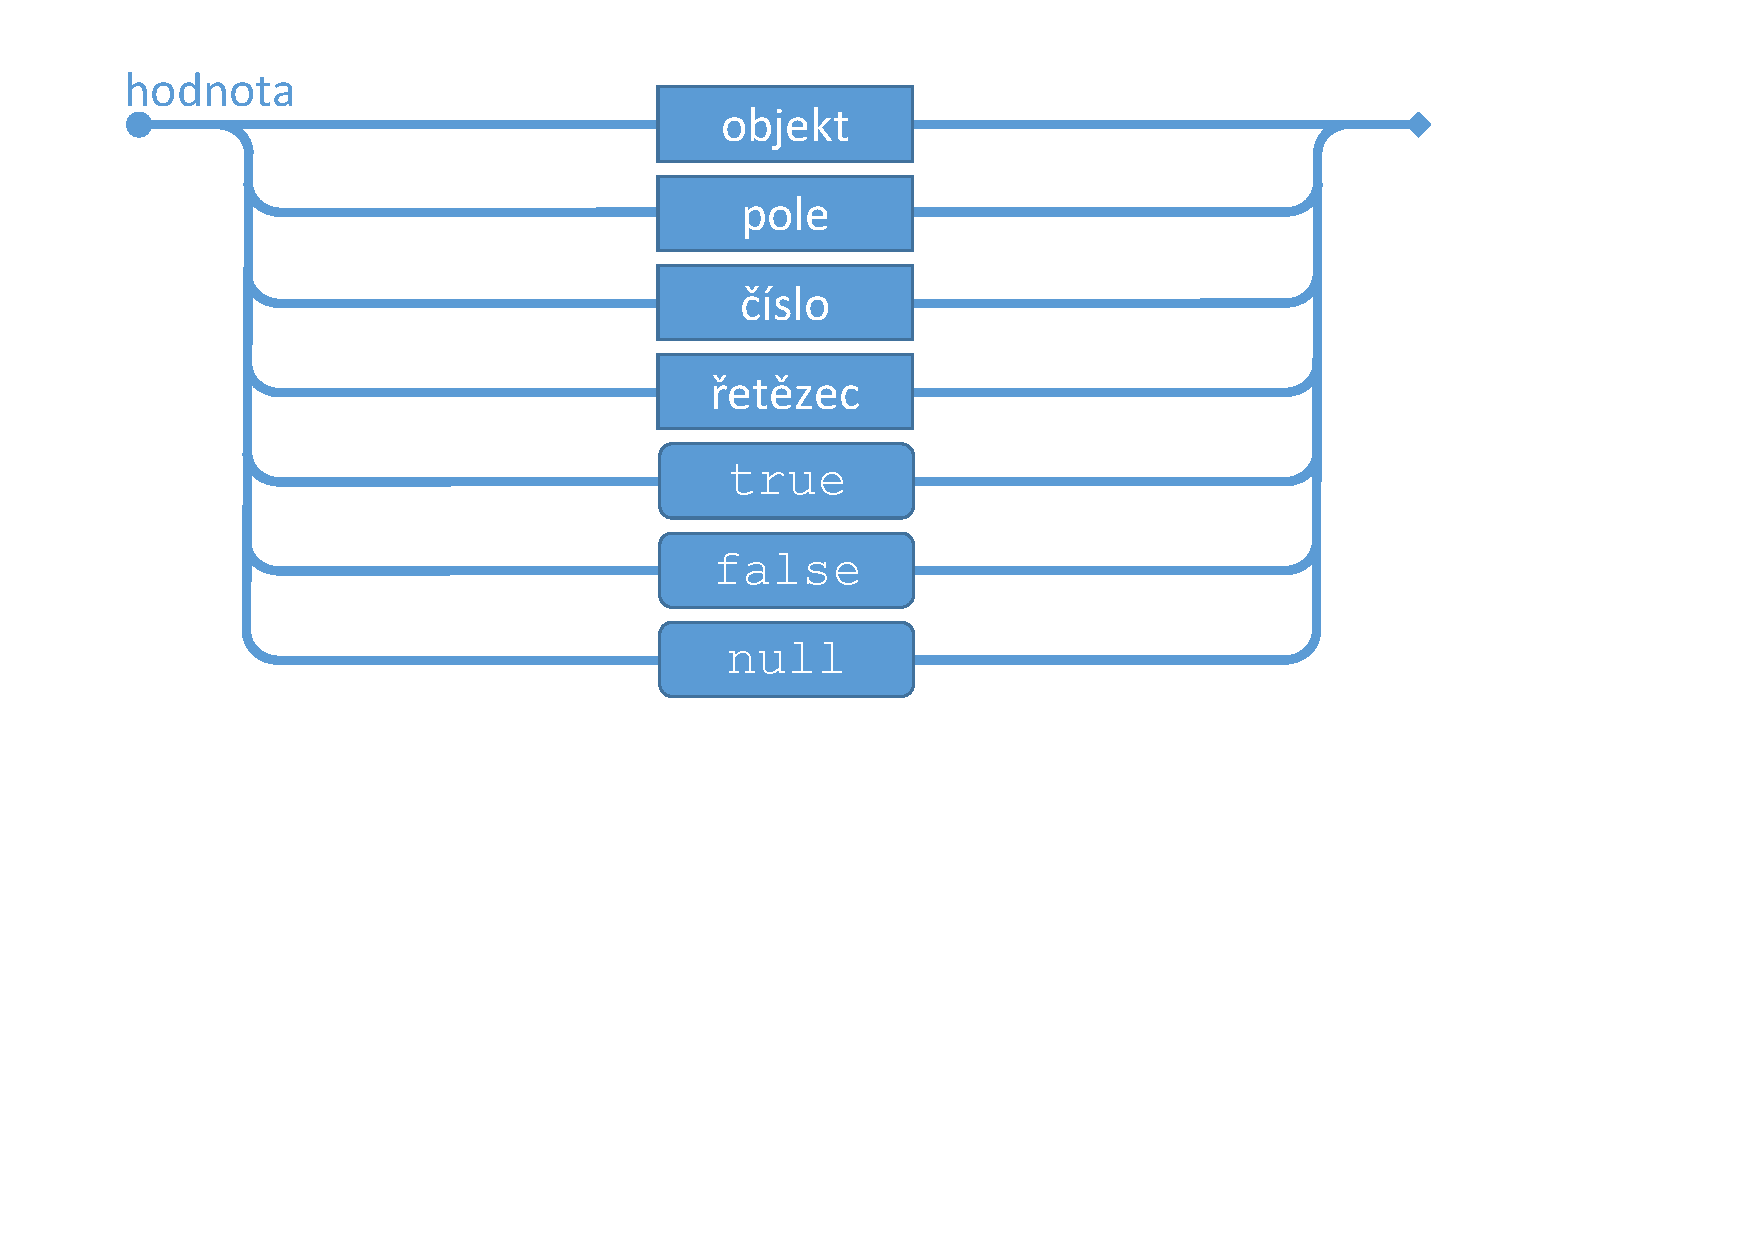
\includegraphics[trim=0 260 90 30, clip, angle=0, width=150mm]{hodnota}
\caption{Struktura hodnoty}
\label{hodnota}
\end{figure}

\subsubsection{Objekty}
Objekt je reprezentován dvojicí složených závorek, uvnitř kterých je žádná nebo více dvojic klíč/hodnota, přičemž klíč je řetězec. Klíč a hodnota jsou odděleny dvojtečkou a jednotlivé dvojice odděluje čárka.

\begin{figure}[!htb]
\centering
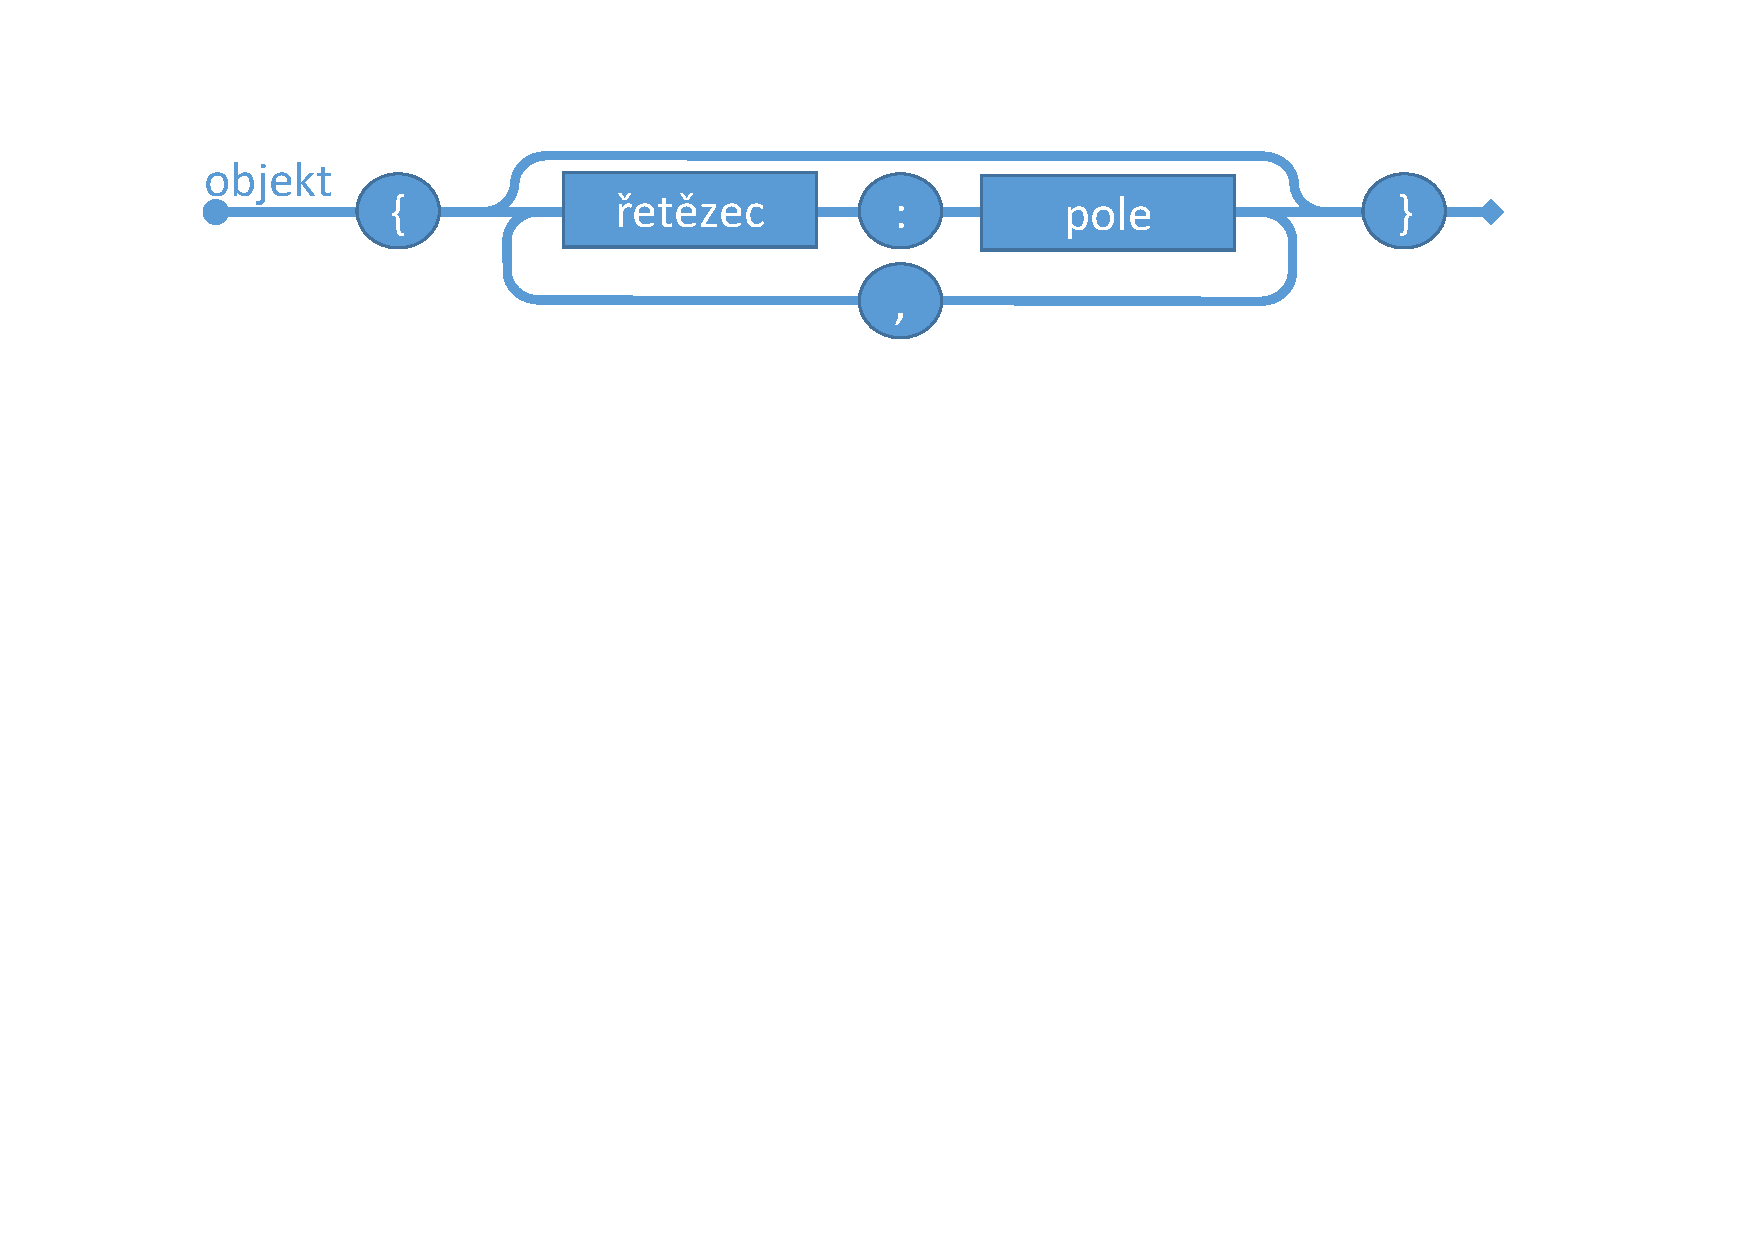
\includegraphics[trim=70 430 80 70, clip, angle=0, width=150mm]{objekt}
\caption{Struktura objektu}
\label{objekt}
\end{figure}

\subsubsection{Pole}
Pole je složeno z dvojice hranatých závorek, mezi kterými může být nula nebo více seřazených hodnot, které jsou odděleny čárkou.

\begin{figure}[!htb]
\centering
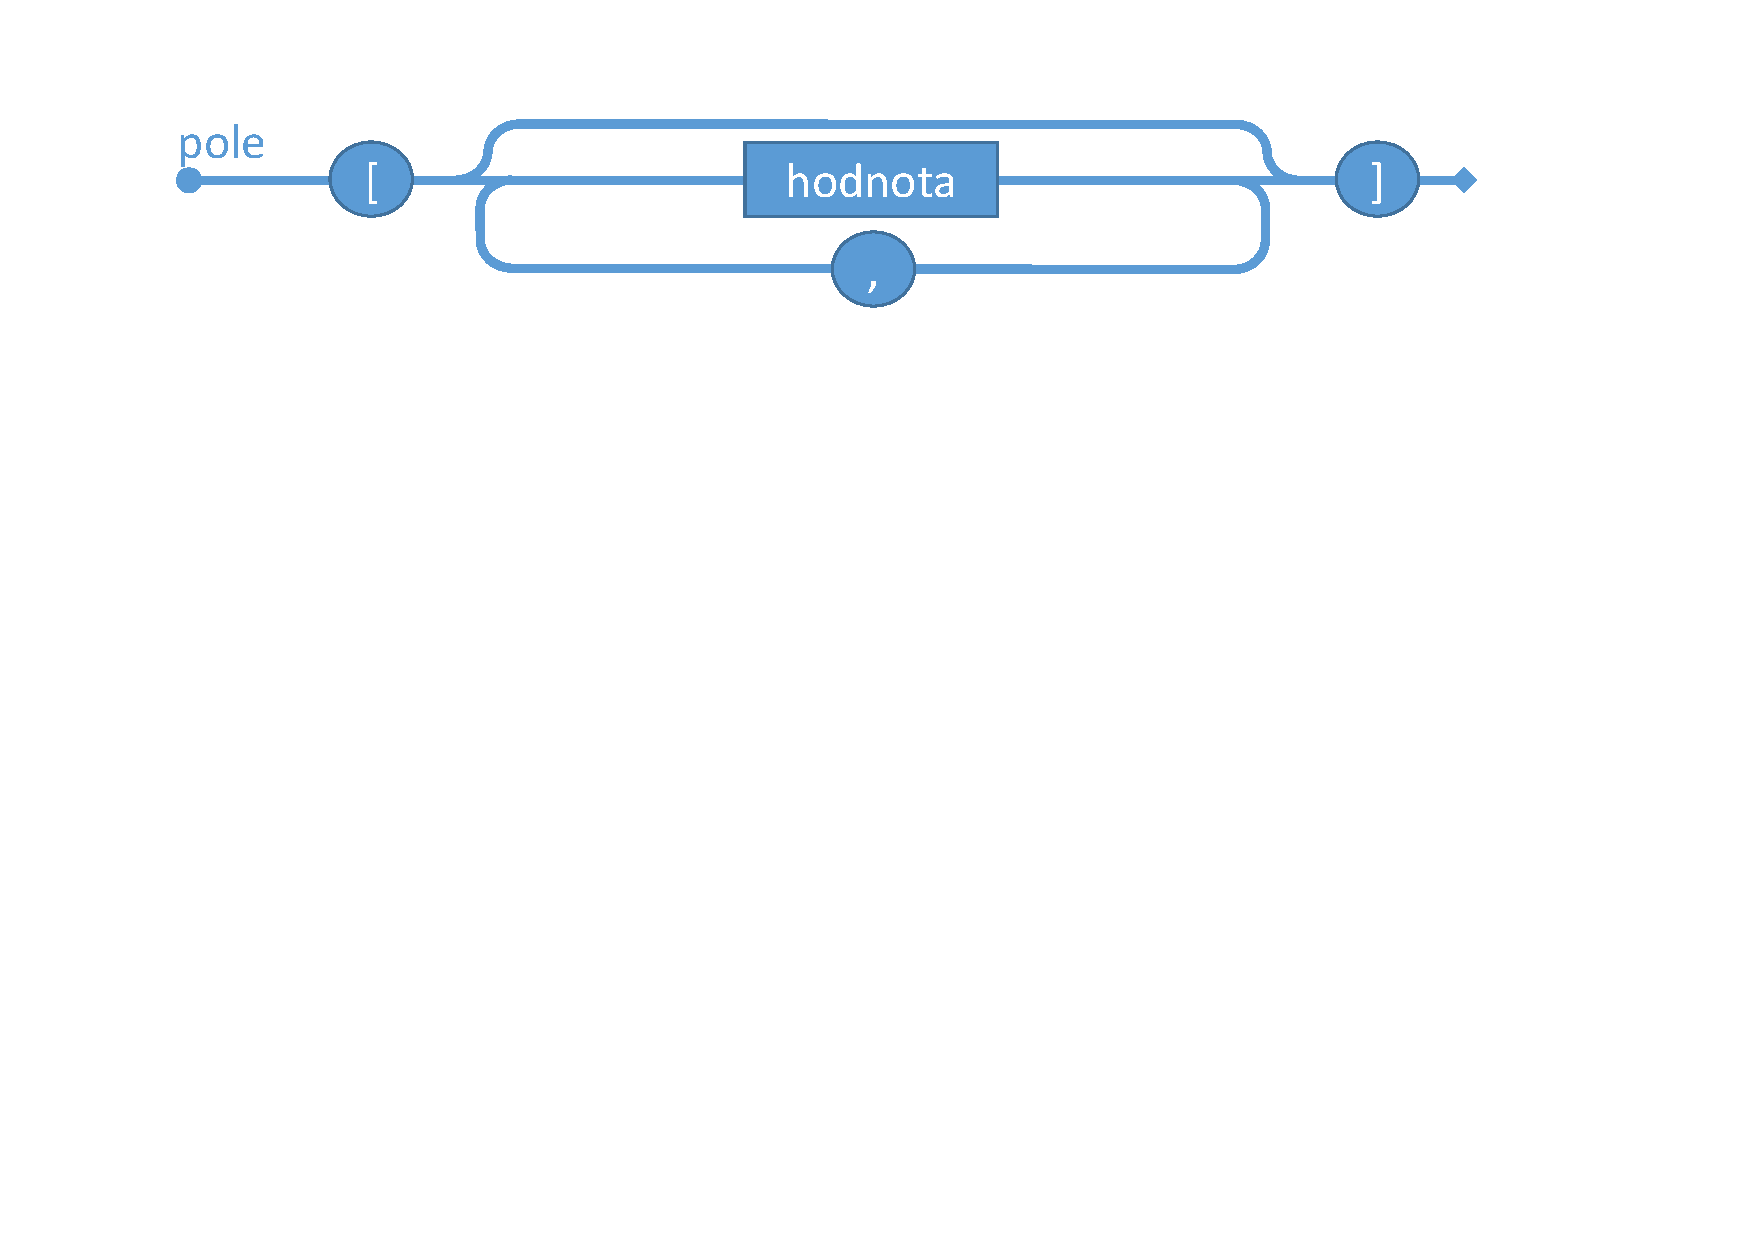
\includegraphics[trim=60 445 90 55, clip, angle=0, width=150mm]{pole}
\caption{Struktura pole}
\label{pole}
\end{figure}

\subsubsection{Čísla}
Čísla jsou v desítkové soustavě (tedy číslice $0 - 9$), záporná čísla jsou uvozena znaménkem \texttt{-} (mínus), desetinná část je oddělena znaménkem \texttt{.} (tečka). Je možný i takzvaný vědecký zápis čísel s použitím symbolů \texttt{e} (malé e) nebo \texttt{E} (velké e) a volitelně lze použít u exponentu znaménka \texttt{+} (plus) nebo \texttt{-} (mínus).

\begin{figure}[!htb]
\centering
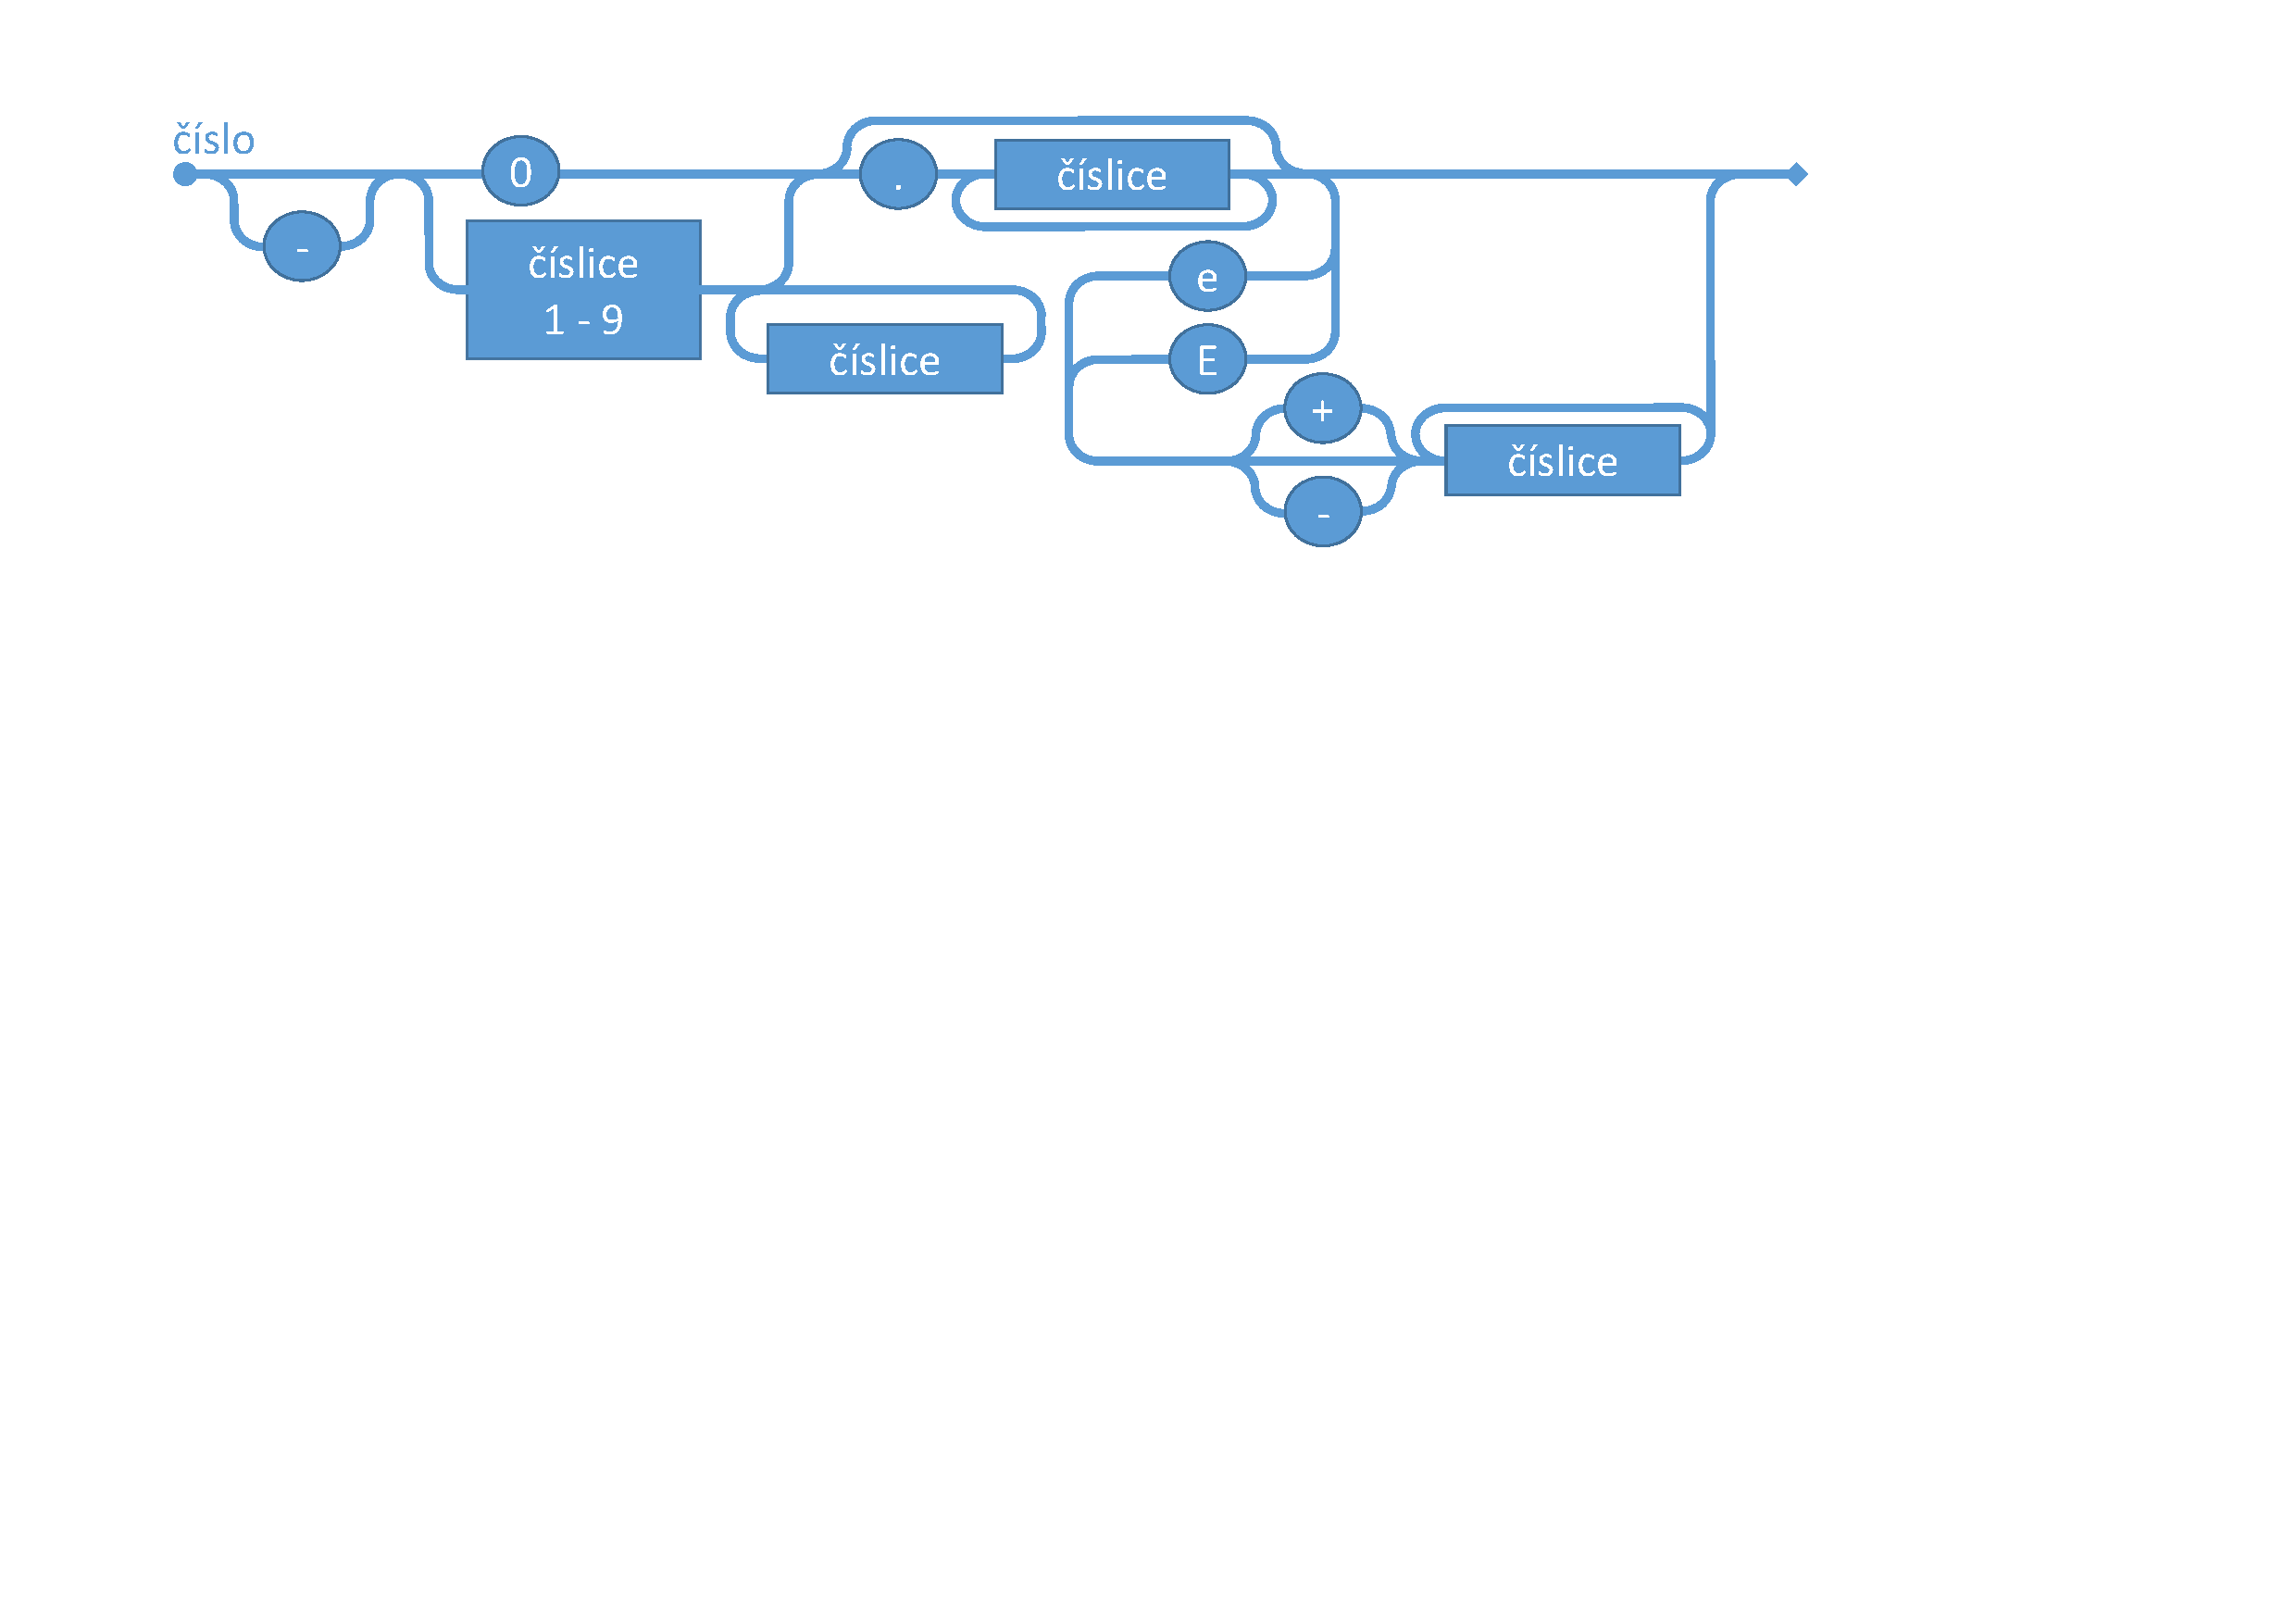
\includegraphics[trim=80 550 240 55, clip, angle=0, width=150mm]{cislo}
\caption{Struktura čísla}
\label{cislo}
\end{figure}

\subsubsection{Řetězce}
Řetězec je posloupnost Unicode znaků uvozená a zakončená znakem \texttt{\textquotedblright} (uvozovky). Mezi uvozovky mohou být zapsány všechny znaky kromě speciálních znaků, které jsou uvozeny tzv. únikovým znakem \texttt{\textbackslash} (zpětné lomítko), těmito znaky jsou například \texttt{\textquotedblright}, \texttt{\textbackslash}, \texttt{t} (znak tabulátoru), \texttt{n} (znak posunu kurzoru na nový řádek) a \texttt{r} (znak posunu kurzoru na začátek řádku, známý jako návrat vozíku) a další. Kompletní výčet je možné vidět na obrázku \ref{retezec} nebo v \cite{json}. Navíc je možné každý znak zapsat pomocí kombinace \texttt{\textbackslash u} a čtyřmístného hexadecimálního čísla odpovídajícího Unicode kódu požadovaného znaku. Řetězec obsahující pouze zpětné lomítko můžeme tedy zapsat následujícími způsoby: \texttt{\textquotedblright\textbackslash\textbackslash\textquotedblright}, \texttt{\textquotedblright\textbackslash u005c\textquotedblright} nebo \texttt{\textquotedblright\textbackslash u005C\textquotedblright} (u hexadecimálních čísel \texttt{A-F} nezáleží na velikosti).

\begin{figure}[!htb]
\centering
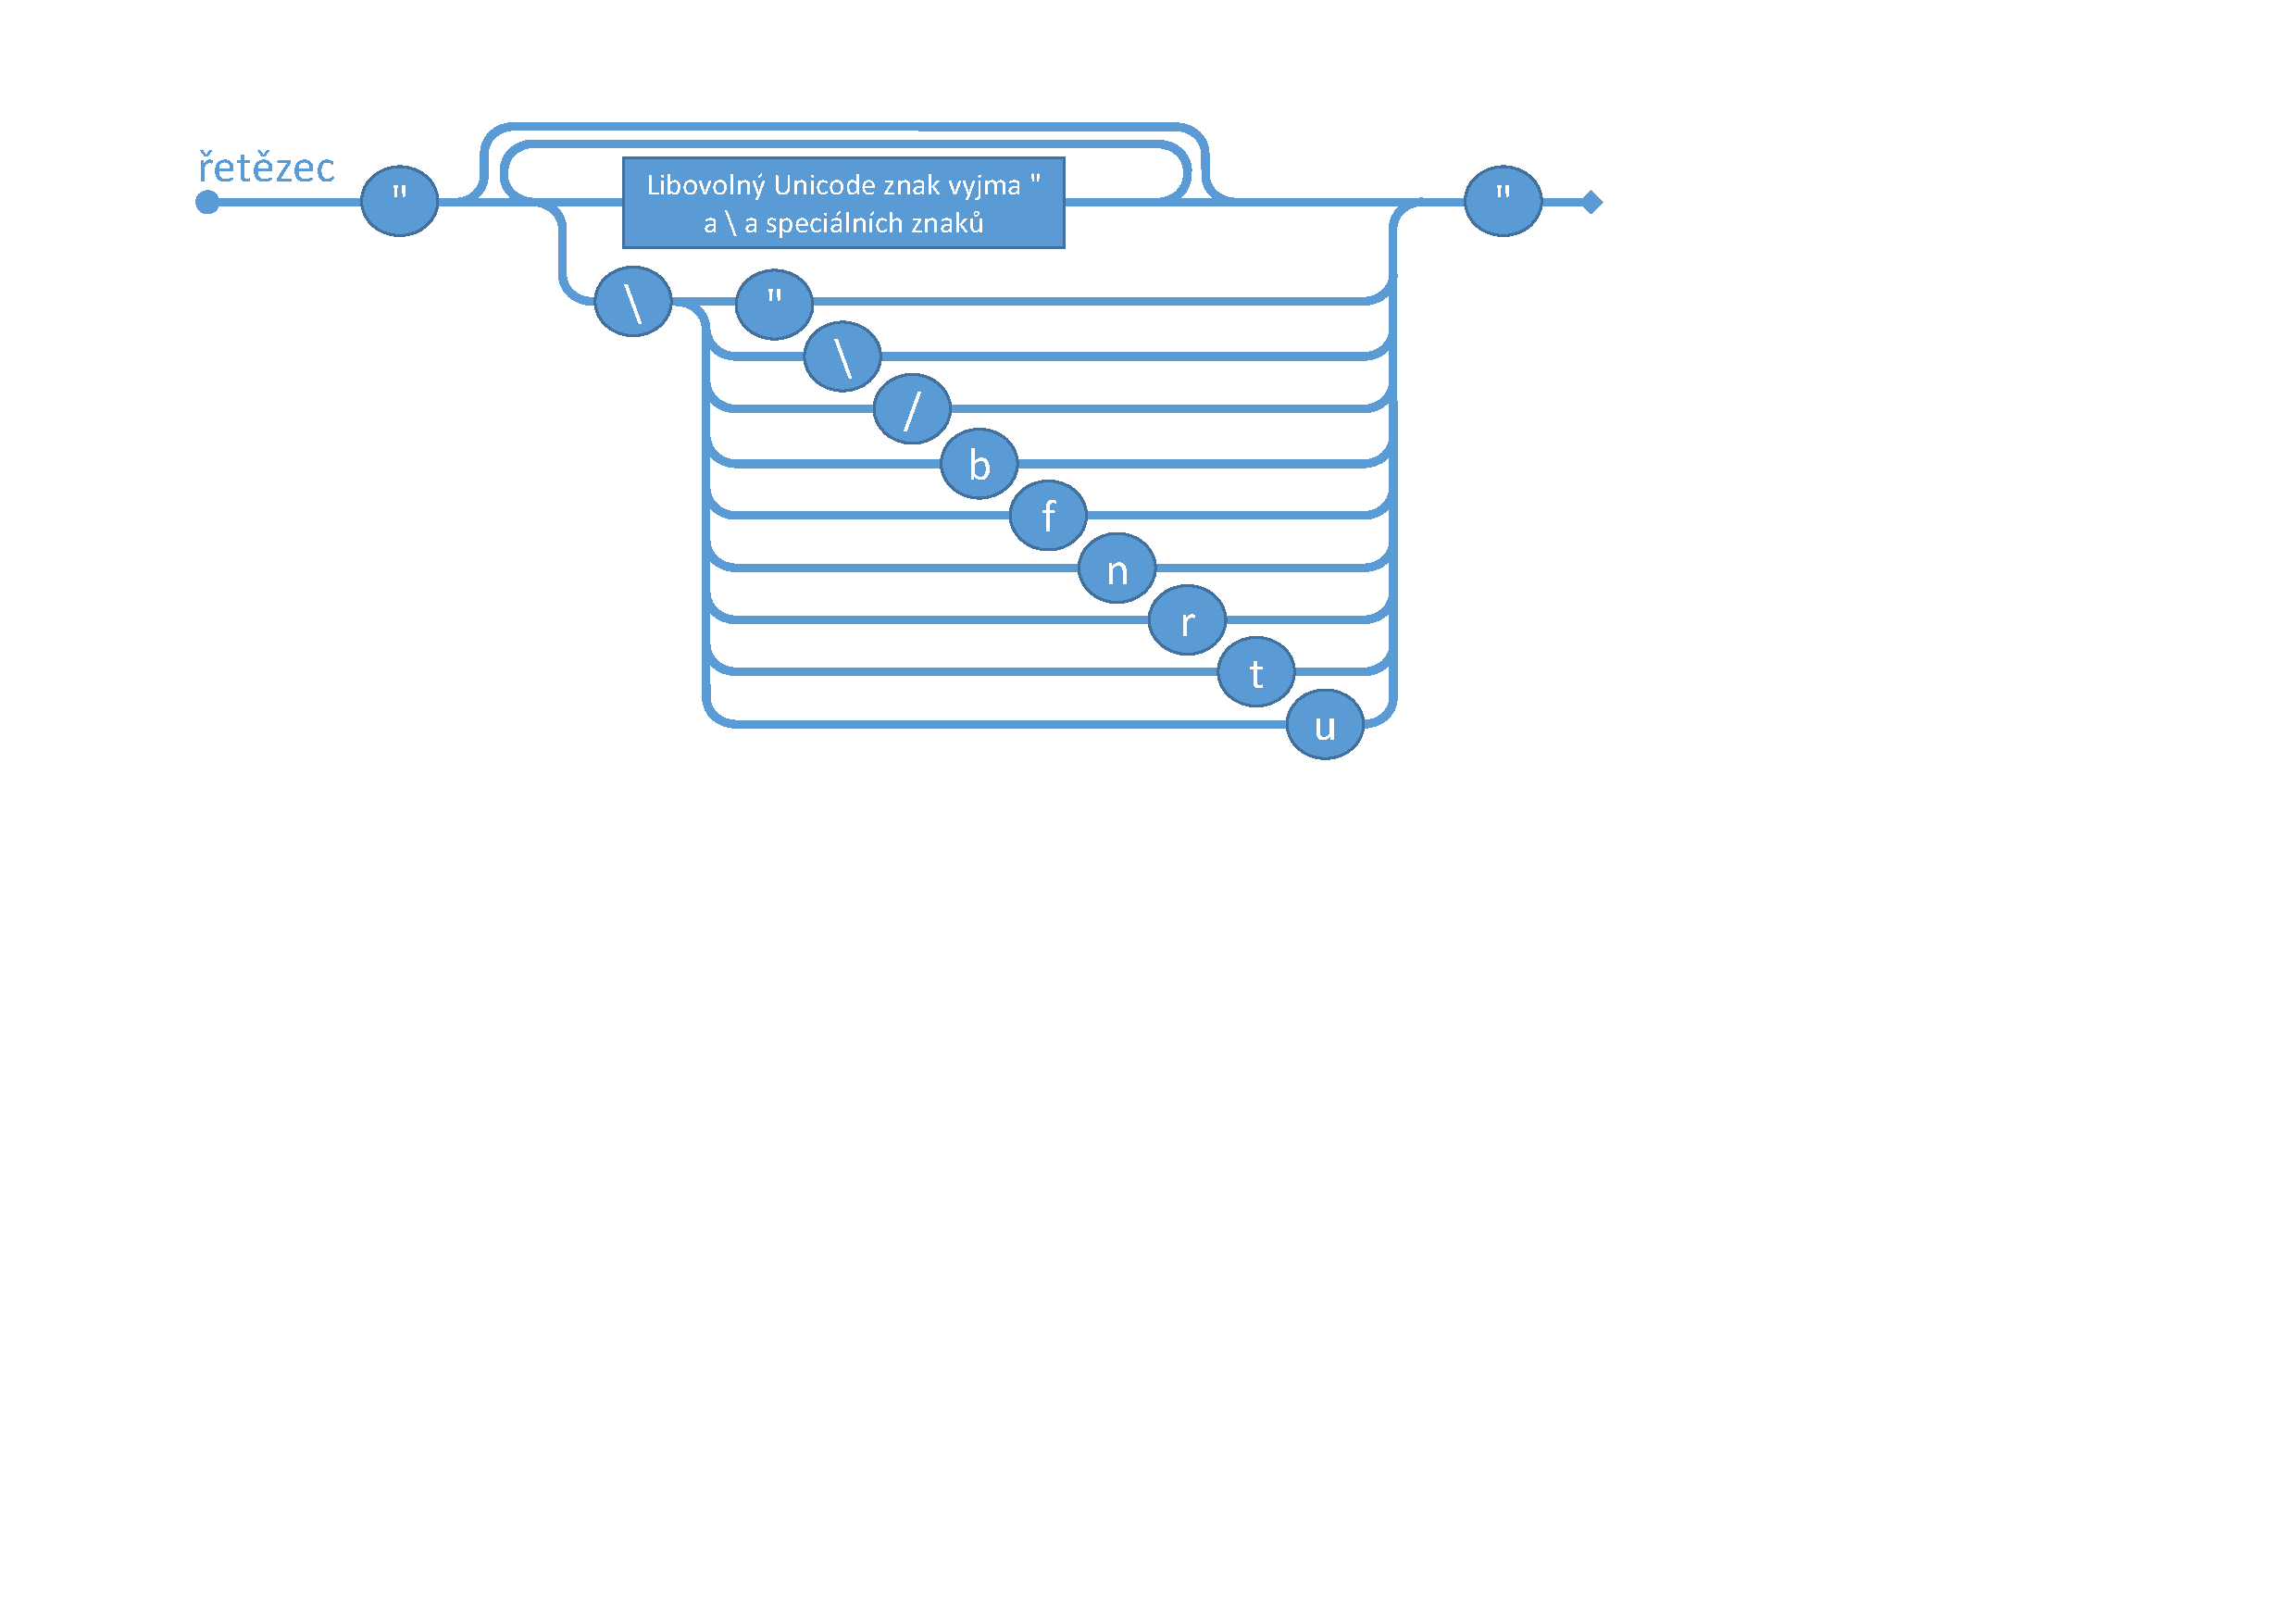
\includegraphics[trim=80 440 360 55, clip, angle=0, width=150mm]{retezec}
\caption{Struktura řetězce}
\label{retezec}
\end{figure}

\subsection{Vzorový příklad}
Stejně jako ve vzorovém příkladu \ref{xmlpriklad} ke XML, je zde popsána postavička Homera Simpsona včetně příbuzných, tentokrát ale v notaci JSON. Jde o objekt složený ze tří atributů, první dva mají hodnoty typu řetězec, k poslednímu \texttt{relatives} ale přísluší hodnota typu pole, ve kterém je vloženo pět příbuzných -- hodnot typu řetězec.

\texttt{\small\{\\
\hspace*{2mm}"firstName": "Homer",\\
\hspace*{2mm}"lastName": "Simpson",\\
\hspace*{2mm}"relatives": [\\
\hspace*{4mm}"Grandpa",\\
\hspace*{4mm}"Marge",\\
\hspace*{4mm}"Bart",\\
\hspace*{4mm}"Lisa",\\
\hspace*{4mm}"Maggie"\\
\hspace*{2mm}]\\
\} }

\section{Vzájemné porovnání XML a JSON}

%Vybrat nějaké argumenty z diskusí a zapsat je tady pro porovnání

Je XML obecně lepší než JSON? Co vlastně dělá jeden formát lepší než jiný? Na toto bylo vedeno již nespočet diskusí. Argumentace obou stran diskuse je obvykle podložena jak teoretickou znalostí formátů, tak i praktickým použitím v reálných projektech. I přesto si myslím, že žádná diskuse nepřinesla jednoznačnou odpověď na výše položenou otázku, což samozřejmě pro některé konkrétní případy použití neplatí a volba jednoho z formátů je nutná nebo alespoň výhodnější. Ze svého zkoumání této problematiky si ale odnáším jeden podstatný závěr, který bych chtěl čtenáři zdůraznit: Vždy záleží na konkrétní situaci. Před samotným rozhodnutím, který z formátů využít, je vhodné zvážit důležité požadavky a do těchto úvah zahrnout klidně i další z existujících datových formátů. Zároveň lze ale říci, že pokud splňuje vybraný formát požadavky, tak ho lze považovat za dostatečný 

Podíváme-li se znovu na vzorové příklady zápisu dat nebo položíme-li si vedle sebe stejná data zapsaná do obou formátů (viz příloha \ref{prilohaPorovnaniXmlJson}), můžeme lehce vidět vzájemnou podobnost. Ve své práci proto vycházím z předpokladu, že jsou oba formáty z hlediska toho, jaká data lze do nich zapsat, ekvivalentní. Respektive budu pro další porovnání používat pouze takový druh dat, který bude tento předpoklad splňovat.  % Obecné seznámení s formáty XML a JSON
\chapter{Komprese dat}
Komprese nebo také komprimace dat je taková transformace dat, která má za cíl úsporu zdrojů při archivaci dat anebo snížení datového toku při přenosu, to vše při současném zachování informace obsažené v datech. Jinými slovy jde o redukci velikosti datových souborů, jehož následkem je úspora paměťových či přenosových kapacit. Postup, při kterém z komprimovaných dat rekonstruujeme data originální, se nazývá dekomprese.

\section{Princip komprese dat}
\label{sekcePrincipKompreseDat}
Data velmi často obsahují tzv. redundantní\footnote{Redundance znamená informační nadbytek, např. vícenásobný výskyt slov v textu.} informaci, toho právě využívá komprese -- data jsou zpracována tak, aby byla redundance minimalizována. Jak lze vidět na obrázku \ref{kompreseDekomprese}, je na vstupní data použita operace komprese. Operací dekomprese dostaneme poté data rekonstruovaná -- v závislosti na použité kompresní metodě a požadavcích získáme buď data přesně odpovídající původním, nebo pouze částečná. Z tohoto hlediska rozlišujeme dva typy kompresních metod: ztrátové a bezeztrátové.

\begin{figure}[!htb]
\centering
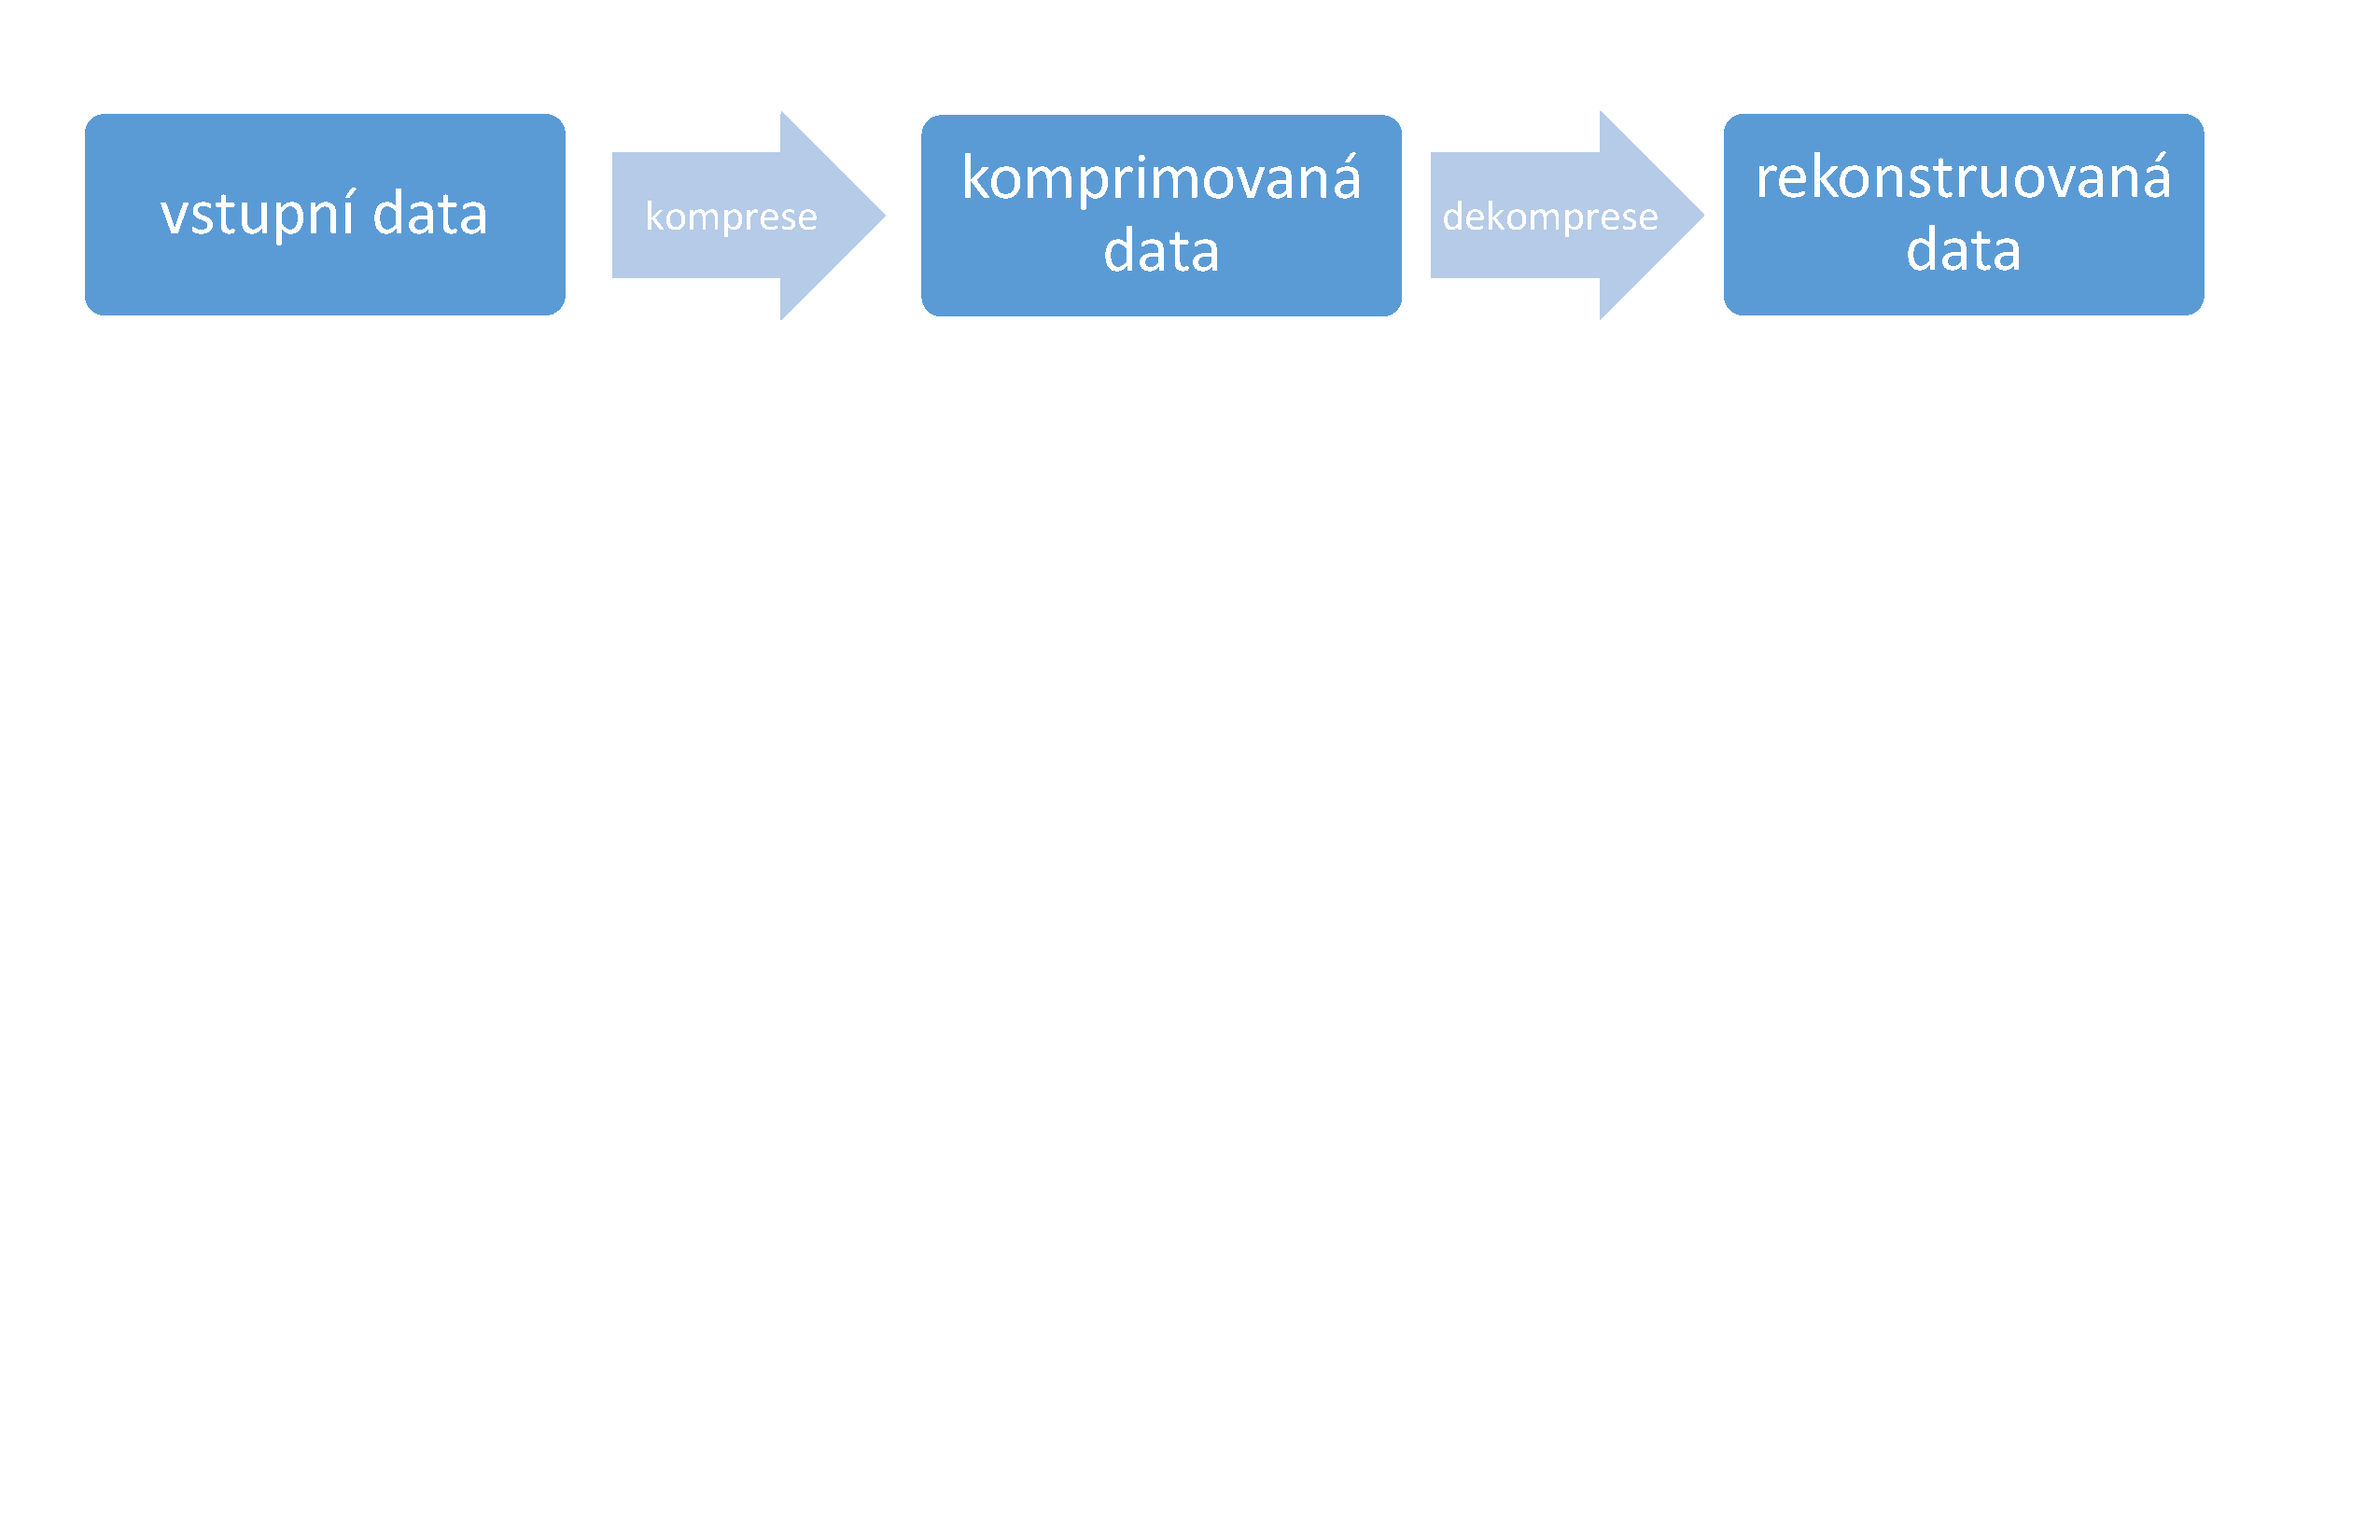
\includegraphics[trim=0 610 60 55, clip, angle=0, width=150mm]{kompreseDekomprese}
\caption{Princip komprese}
\label{kompreseDekomprese}
\end{figure}

\section{Typy kompresních metod}
Jak název napovídá, při ztrátové kompresi ztratíme část informace obsaženou v původních datech, respektive jsou původní data pouze aproximována.  Toto nám nemusí vadit na\-pří\-klad u obrázků, zvuku a videí, kde je využito nedokonalosti lidských smyslů. Lidské ucho nedokáže například slyšet velmi vysoké frekvence. Má smysl v datech určených k poslechu zachovávat informaci, kterou nemůže člověk slyšet? Častá odpověď je \uv{ne}. Tohoto principu využívá mnoho kompresních metod, například známý zvukový formát MP3. Odstraněním nepotřebné informace z dat je dosaženo ještě větší redukce objemu. 

Naopak v případě bezeztrátových metod je při kompresi zachována veškerá informace a při dekompresi
jsou rekonstruována původní data. Těchto metod se využívá převážně tam, kde není možné původní data jakkoliv pozměnit. Například data ve formátech XML a JSON, kterým se věnuji v této práci, si nemůžeme dovolit pozměnit (přestanou mít původní význam), nebo dokonce ztratit.

\section{Charakteristika komprese}
Kompresní algoritmy lze hodnotit z mnoha různých úhlů pohledu. Můžeme měřit složitost algoritmu, rychlost, jakou jsou data komprimována a dekomprimována (to může být ovlivněno výkonem stroje, na kterém algoritmus běží), jak moc odpovídají rekonstruovaná data původním atd.
Jednou z nejčastějších charakteristik je, logicky ze smyslu komprese vy\-plý\-va\-jí\-cí, tzv. kompresní poměr, který vyjadřuje velikost komprimovaných dat vůči původním, lze ho zapsat následujícím  vztahem:
\begin{equation}
\texttt{kompresní poměr} = \frac{\texttt{délka původních dat}}{\texttt{délka komprimovaných dat}}.
\end{equation}

Další sledovanou charakteristikou je tzv. úspora místa, která je vyjádřena jako:
\begin{equation}
\texttt{úspora místa} = \texttt{1 - kompresní poměr$^{-1}$}.
\end{equation}

Mějme například 2D obrázek o velikosti $256\times256$ pixelů, který zabírá 65536 bytů. Obrázek zkomprimujeme a zabírá-li komprimovaná verze 16384 bytů, můžeme říct, že kompresní poměr je $4:1$ a úspora místa 75 \%. 

\section{Míra informace v datech}
Než se budeme moci věnovat jednotlivým kompresním metodám, připomeňme stručně myšlenky z teorie informace, které poskytly základ pro rozvoj metod bezeztrátové komprese. V této části předpokládám čtenářovu znalost základů teorie pravděpodobnosti a~statistiky.

Informační entropie\footnote{Nazývaná též Shannonova po Claudu E. Shannonovi, který zformuloval klíčové poznatky.}, jakožto míra neurčitosti v datech, nám pomůže lépe porozumět principům komprese. Představme si dva zdroje (označím je $\mathbf{Z}_1$ a $\mathbf{Z}_2$), které produkují zprávy složené ze symbolů (znaků) zdrojové abecedy $\mathbb{A} = \{\alpha, \beta, \gamma, \delta\}$. Oba zdroje generují znaky zprávy náhodně, pro zdroj $\mathbf{Z}_1$ však platí, že mají všechny znaky stejnou pravděpodobnost výskytu a to 0,25. Pro zdroj $\mathbf{Z}_2$ jsou pravděpodobnosti výskytu popsány v tabulce \ref{pstVyskytu}. Který ze zdrojů produkuje více informace?

\begin{table}[!htb]
\centering
\begin{tabular}{|c|c|}
\hline
Znak & Pravděpodobnost výskytu\\
\hline
$\alpha$ & $p_\alpha = 0,5$\\
$\beta$ & $p_\beta = 0,3$\\
$\gamma$ & $p_\gamma = 0,1$\\
$\delta$ & $p_\delta = 0,1$\\
\hline
\end{tabular}
\caption{Pravděpodobnost výskytu znaků abecedy $\mathbb{A}$ ve zdroji $\mathbf{Z}_2$}
\label{pstVyskytu}
\end{table}

Claude E. Shannon si tuto otázku položil následujícím způsobem. Jaký je nejmenší počet otázek s odpověďmi ano nebo ne, které musíme zodpovědět, abychom byli schopni rozhodnout, jaký je následující znak každého zdroje? Odpovědí na tuto zdánlivě složitou otázku je vyhledávací algoritmus binární vyhledávání. Nejefektivnějším způsobem je v každém kroku položit takovou otázku, která rozdělí prohledávaný interval na dvě poloviny z hlediska pravděpodobnosti. Pro zobrazení, jaké otázky pokládat a v jakém pořadí, můžeme využít binární rozhodovací stromy (viz obrázky \ref{rozhodovaciStromZ1} pro zdroj $\mathbf{Z}_1$ a \ref{rozhodovaciStromZ2} pro zdroj $\mathbf{Z}_2$). Čteme je zleva doprava, v uzlech jsou otázky, hrany odpovídají odpovědím a v listech jsou příslušné znaky.

\begin{figure}[!htb]
\centering
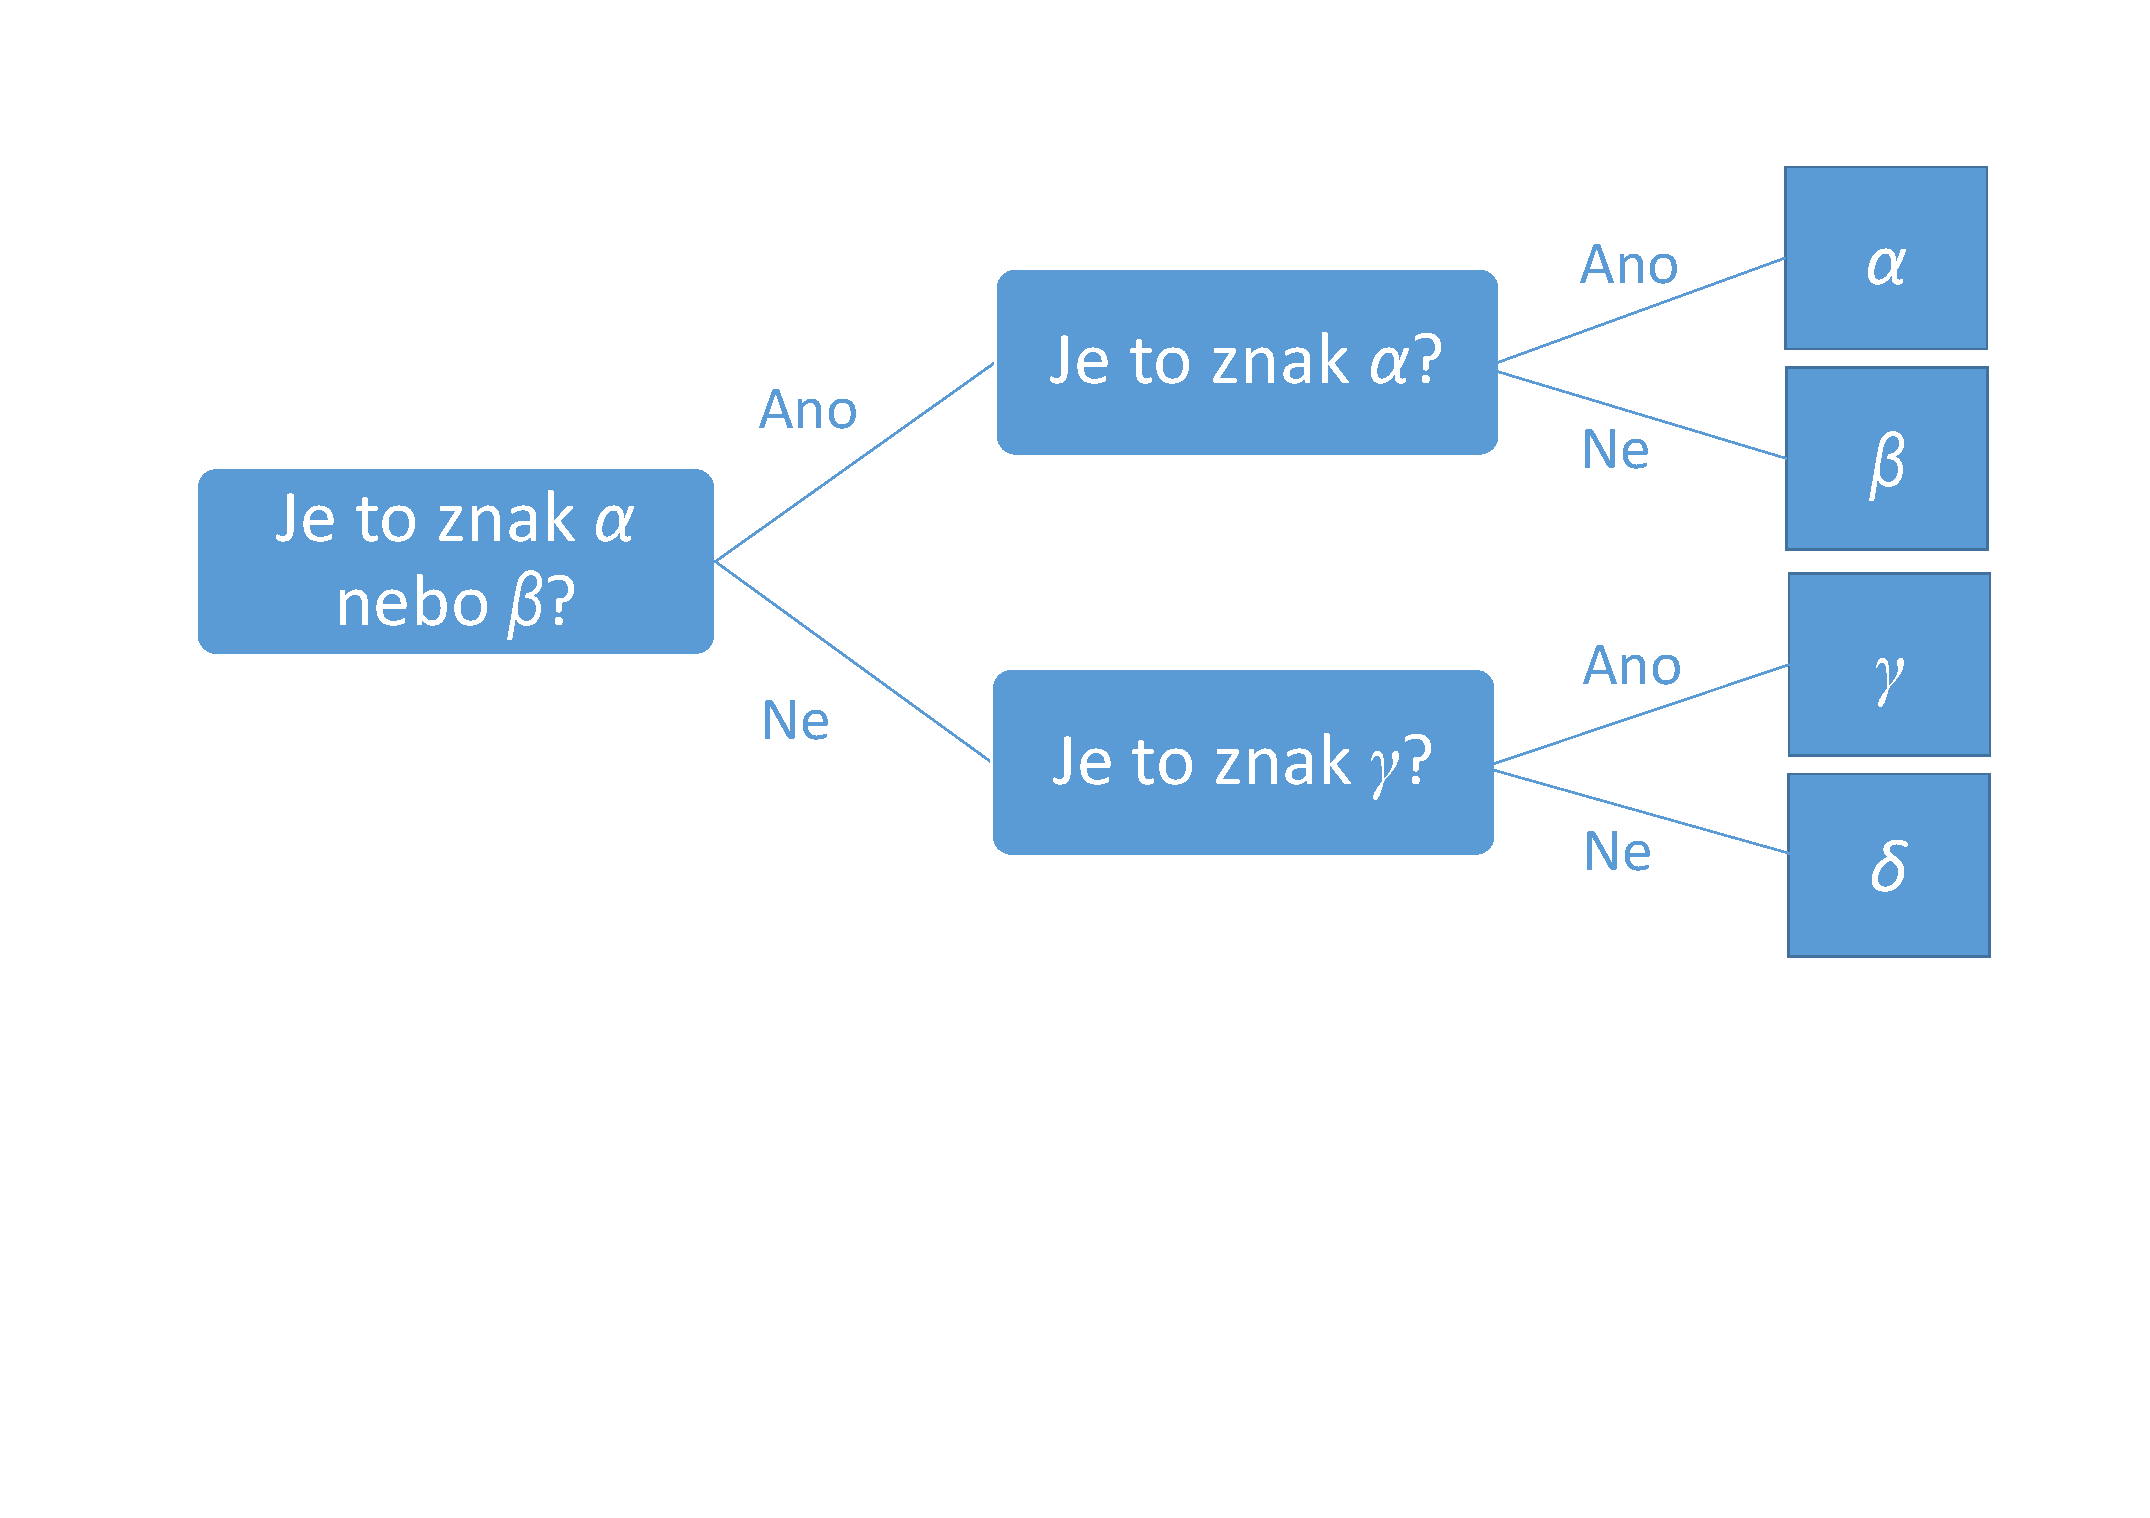
\includegraphics[trim=50 270 50 70, clip, angle=0, width=120mm]{rozhodovaciStromZ1}
\caption{Binární rozhodovací strom pro zdroj $\mathbf{Z}_1$}
\label{rozhodovaciStromZ1}
\end{figure}

\begin{figure}[!htb]
\centering
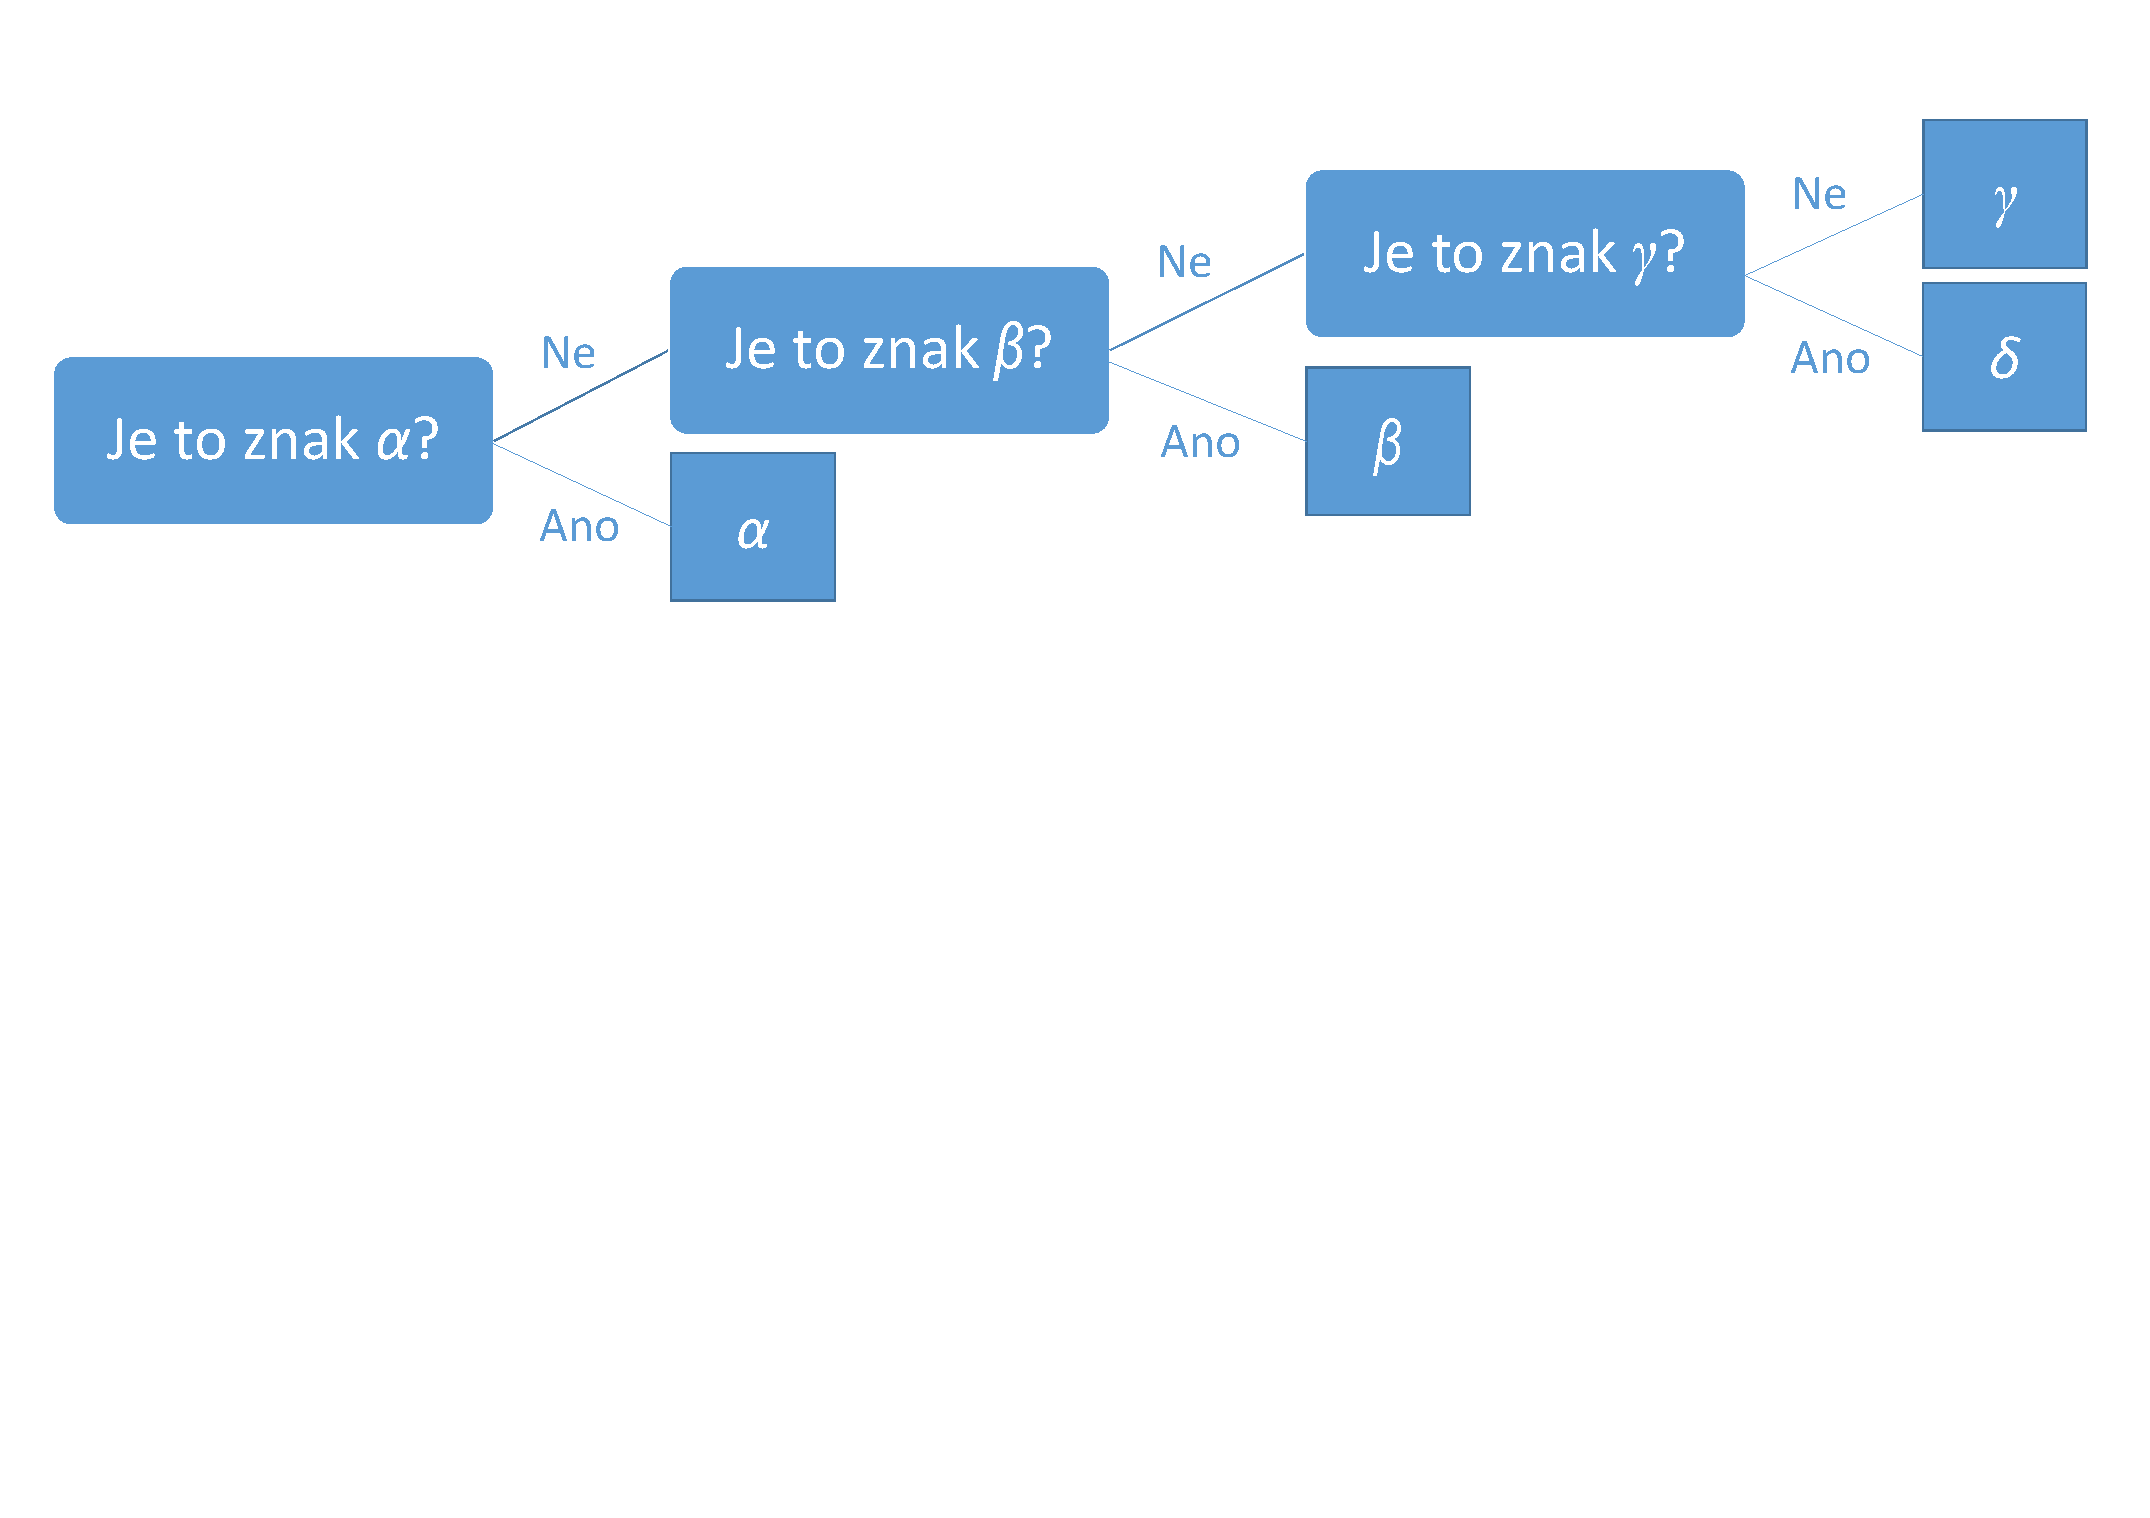
\includegraphics[trim=20 420 20 40, clip, angle=0, width=150mm]{rozhodovaciStromZ2}
\caption{Binární rozhodovací strom pro zdroj $\mathbf{Z}_2$}
\label{rozhodovaciStromZ2}
\end{figure}

Průměrný počet otázek na zjištění jednoho znaku (tento počet označím $\bar{q}$) pokládaných tímto způsobem odpovídá pravděpodobnostem výskytu jednotlivých znaků a lze jej vy\-po\-čí\-tat jako $\bar{q} = \sum_{a \in \mathbb{A}} \#a \cdot p_a$, kde $\#a$ je počet otázek pro zjištění, že jde o znak $a$, a $p_a$ je pravděpodobnost výskytu znaku $a$. Pro zdroj $\mathbf{Z}_1$ dostaneme $\bar{q}_1 = 2p_\alpha + 2p_\beta + 2p_\gamma + 2p_\delta =$ $=2\cdot0,25 + 2\cdot0,25 + 2\cdot0,25 + 2\cdot0,25 = 2$, tedy 2 otázky na znak, a pro zdroj $\mathbf{Z}_2$ dostaneme podobně $\bar{q}_2 = 1p_\alpha + 2p_\beta + 3p_\gamma + 3p_\delta =1\cdot0,5 + 2\cdot0,3 + 3\cdot0,1 + 3\cdot0,1 = 1,7$, tedy $1,7$ otázky na znak.

To znamená, že budeme-li se ptát na 1000 znaků u obou zdrojů, budeme muset položit 2000 otázek ke zjištění znaků ze zdroje $\mathbf{Z}_1$ a 1700 otázek ke zjištění znaků ze zdroje $\mathbf{Z}_2$. Výstup zdroje $\mathbf{Z}_2$ obsahuje méně překvapení, nebo lépe neurčitosti, než výstup zdroje $\mathbf{Z}_1$. Hovoříme o tom, že výstup zdroje $\mathbf{Z}_2$ poskytuje méně informace než výstup zdroje $\mathbf{Z}_1$.

\subsection{Entropie informačního zdroje}
V Shannonově teorii je definice zdroje informace prakticky totožná s definicí pravdě\-po\-do\-bno\-stní\-ho prostoru, tj. trojice $(\mathcal{X},\mathcal{S},p)$, kde $\mathcal{X}$ je množina elementárních jevů (zpráv), $\mathcal{S}$ je třída náhodných jevů ($\sigma$-algebra podmnožin $\mathcal{X}$) a $p$ je pravděpodobnostní míra na $\mathcal{S}$. \cite{teorieInformace}

Pro nás bude modelem zdroje informace diskrétní pravděpodobnostní prostor $(\mathcal{X},p(x))$, který generuje zprávu $X$, jež je náhodnou veličinou s výběrovým prostorem $(\mathcal{X}, px(x))$. Mezi zprávou $X$ a zdrojem $(\mathcal{X}, p(x))$ panuje ekvivalence, značíme $X \thicksim (\mathcal{X}, p(x))$. Základním pojmem teorie informace je entropie $H(X)$ zdroje $X$, jde o číslo, kterým charakterizujeme, jak obtížné je předpovědět hodnotu dané náhodné veličiny $X$, tj. zprávu, kterou vyprodukuje daný zdroj informace $X \thicksim (\mathcal{X}, p(x))$. Následuje formální definice entropie. \cite{teorieInformace}

\begin{defi}
Entropie zdroje informace $X \thicksim (\mathcal{X}, p(x))$ je veličina $$H(X) = -\sum_{x \in \mathcal{X}} p(x)\log p(x),$$ kde $0 \log 0 = \lim_{t \to 0_+} t \log t = 0$.
\end{defi}

\subsection{Entropie a komprese}
Když chceme komprimovat digitální data, musíme je rozdělit na malé kousky, např. obrázek na pixely, textová data na znaky. To nám umožní zpracovat tato data jako posloupnost symbolů. Jednotlivé symboly pak můžeme reprezentovat s použitím nějakého kódu. Umíme-li zprávy vysílat a přijímat pouze v binární soustavě, vytvoříme kód\footnote{Takové binární kódy provází lidstvo již velice dlouho, např. kouřové signály, kódování znaků v Morseově abecedě.} složený ze znaků kódové abecedy $\mathbb{B} = \{0,1\}$.

Vraťme se nyní zpět k abecedě $\mathbb{A}$ a představme si zdroj $\mathbf{Z}$, který generuje zprávy složené ze znaků abecedy $\mathbb{A}$. Tento zdroj má pravděpodobnosti výskytu jednotlivých znaků odpovídající zdroji $\mathbf{Z}_2$, což my zatím ale nevíme. Jako příklad můžeme mít za úkol komprimovat text obsahující 1000 znaků vygenerovaných zdrojem $\mathbf{Z}$. V takovém případě intuitivně přiřadíme jednotlivým zdrojovým znakům nejkratší možná kódová slova viz kód $\kappa_1$ v tabulce \ref{kodovaSlovaZ1}. Tato slova mají délku 2, což znamená, že potřebujeme průměrně 2 bity na znak. 

\begin{table}[!htb]
\centering
\begin{tabular}{|c|l|}
\hline
Zdrojový znak & Kódové slovo\\
\hline
$\alpha$ & 11\\
$\beta$ & 10\\
$\gamma$ & 01\\
$\delta$ & 00\\
\hline
\end{tabular}
\caption{Kód $\kappa_1$ pro zdroj $\mathbf{Z}_1$}
\label{kodovaSlovaZ1}
\end{table}

Pokud analýzou zdroje $\mathbf{Z}$ ale zjistíme, že pravděpodobnosti výskytu odpovídají zdroji $\mathbf{Z}_2$ (viz tabulka \ref{pstVyskytu}), můžeme znakům přiřadit jiná kódová slova (viz tabulka \ref{kodovaSlovaZ2}), která budou brát ohled na nové pravděpodobnosti výskytu. Tento kód $\kappa_2$ je tzv. Huffmanův kód (viz kapitola 3 v \cite{teorieKodovani}) a potřebuje průměrně 1,7 bitu na znak, způsob jeho vytvoření je popsán v části \ref{huffmanovoKodovani} nebo v \cite{teorieKodovani}.

\begin{table}[!htb]
\centering
\begin{tabular}{|c|l|}
\hline
Zdrojový znak & Kódové slovo\\
\hline
$\alpha$ & 1\\
$\beta$ & 01\\
$\gamma$ & 000\\
$\delta$ & 001\\
\hline
\end{tabular}
\caption{Kód $\kappa_2$ pro zdroj $\mathbf{Z}_2$}
\label{kodovaSlovaZ2}
\end{table}

Podíváme-li se na obrázky \ref{rozhodovaciStromZ1} a \ref{rozhodovaciStromZ2} a příslušný výpočet průměrného počtu otázek na zjištění znaku, můžeme vidět jisté souvislosti. Například když slova Ano/Ne na hranách rozhodovacího stromu nahradíme čísly 1, resp. 0, dostaneme čtením od kořene k listům odpovídající kódová slova. Stejně tak průměrný počet otázek na zjištění znaku odpovídá střední délce zvoleného kódování (viz definice 7 v \cite{teorieKodovani}).

K jaké úspoře dojde? K zakódování 1000 znaků výše zmíněného textu pomocí kódu $\kappa_1$ potřebujeme 2000 bitů, ale při použití kódu $\kappa_2$ nám bude stačit pouze 1700 bitů. Úspora je tedy 300 bitů. Na otázku, zda je možné tuto úsporu ještě zvýšit, nelze odpovědět jenom ano nebo ne. Pokud zkrátíme délku některých kódových slov v kódu $\kappa_2$, stane se zakódovaná zpráva dvojznačnou a zpětně nedekódovatelnou. Kódujme například znak $\delta$ kódovým slovem 0, potom sekvence 01 může znamenat jak $\delta\alpha$, tak i $\beta$. Abychom odstranili tento problém, museli bychom mezi kódová slova vložit oddělovač, čímž ale zakódovanou zprávu prodloužíme a k požadované úspoře nedojde.

Již Claude E. Shannon tvrdil, že komprese má limit a tím je vždy entropie zdrojové zprávy. Čím je entropie nižší, tím vyšší je možnost komprese. Naopak čím je entropie vyšší, kvůli nepředvídatelnosti, schopnost komprese se snižuje. Pokud bychom chtěli komprimovat až za tento limit, museli bychom nutně část informace vypustit, což je ale přesně princip ztrátové komprese, kterou si nemůžeme vždy dovolit.  % Komprese dat
\chapter{Statistické techniky komprese}
Statistické kompresní metody využívají znalosti tzv. pravděpodobnostního modelu komprimovaných dat. Modelem může být například četnost výskytu jednotlivých symbolů v textu. Účinnost komprese je závislá na schopnosti co nejpřesněji modelovat zpracovávaná data. Čím více se model přibližuje realitě, tím je účinnost komprese vyšší. A naopak.

\section{Pravděpodobnostní model}
\label{pravdepodobnostniModel}
Pravděpodobnostní model přiřazuje pravděpodobnosti výskytu symbolům ve zdrojové zprávě. Na tomto základě například Huffmanovo kódování (viz \ref{huffmanovoKodovani}) přiřazuje symbolům, které se v datech objevují častěji (mají vyšší pravděpodobnost výskytu), kratší kódová slova.

Podle toho, jakým způsobem model vzniká, ho můžeme označit jako statický, semiadaptivní, nebo adaptivní.

\subsection{Statický model}
Tento model je při implementaci kompresní metody a při použití se již nijak nemění. Výhodou je rychlost a jednoduchost vytvoření modelu. Například v případě, že budeme zpracovávat výstup pouze jednoho známého zdroje, se tímto způsobem vyhneme opakovanému vytváření modelu, které by vedlo ke stejným, nebo alespoň velmi podobným výsledkům. V opačném případě ale model nemusí datům vůbec odpovídat, čímž bude dosažená účinnost komprese velice nízká.

\subsection{Semiadaptivní model}
Komprimovaná data jsou jedním průchodem statisticky zpracována a následně je vytvořen odpovídající model. K samotné kompresi je ale nutný ještě druhý průchod daty s již vytvořeným modelem. Aby bylo možné data dekomprimovat, je nutné připojit model k datům. Model je sice přesný, ale velikost zkomprimované zprávy je větší o model. Navíc přístup s dvěma průchody daty činí tyto algoritmy neefektivními a v praxi se moc nepoužívají.

\subsection{Adaptivní model}
Tento mode vzniká v průběhu zpracování dat a je postupně aktualizován. To platí i pro dekompresní algoritmus, ten vytváří model stejně jako kompresní algoritmus z části textu, kterou již dekomprimoval. Díky tomu není nutné model připojovat k datům a také procházet data dvakrát.

\section{Semiadaptivní Huffmanovo kódování}
\label{huffmanovoKodovani}
Huffmanovo kódování je jednou z nejstarších kompresních technik, kterou publikoval již v roce 1952 David A. Huffman. Semiadaptivní dvouprůchodová verze byla od svého vzniku podrobena dalšímu výzkumu a postupně vylepšena až na adaptivní. Je založeno na dvou vlastnostech nejkratších prefixových (jednoznačně dekódovatelných) kódů \cite{introductionToDataCompression}:

\begin{enumerate}
\item Symbolům s vyšší pravděpodobností výskytu jsou přiřazována kratší kódová slova.
\item Dvěma symbolům s nejmenší pravděpodobností výskytu jsou přiřazována kódová slova stejné délky.
\end{enumerate}

Algoritmus nejprve seřadí symboly sestupně podle pravděpodobnosti výskytu a poté z nich v krocích konstruuje strom od listů ke kořeni. V každém kroku jsou vybrány dva symboly s nejmenší pravděpodobností výskytu, z nich je vytvořen nový uzel, který je brán jako symbol s kumulovanou pravděpodobností odpovídající součtu dílčích pravděpodobností. Kroky opakujeme až do vybrání všech symbolů, kdy je kumulovaná pravděpodobnost výskytu rovna 1. Nakonec ohodnotíme hrany vystupující z uzlu vlevo číslem 0 a vpravo číslem 1. Kódová slova získáme čtením stromu od kořene k listům. \cite{dataCompression}, \cite{introductionToDataCompression}

\subsection{Postup kódování a dekódování zprávy}
Při kódování zprávy zapisujeme na výstup kódová slova odpovídající čteným symbolům. Naopak při dekódování procházíme strom od uzlu k listům tak, jak jsou čteny jednotlivé znaky kódových slov. Pokud dojdeme do listu, přečetli jsme jeden původní symbol a můžeme jej vypsat.

\subsection{Vzorový příklad}
Postup lze nejlépe prezentovat na příkladu. Mějme za úkol zakódvat zprávu \uv{MISSISSIPPI} pomocí semiadaptivního Huffmanova kódování. Výsledný strom je zobrazen na obrázku \ref{semiHuffmanStrom}, celá konstrukce pak v příloze \textcolor{red}{reference na konstrukci stromu v příloze}. Místo pravděpodobností výskytu jsou použity absolutní četnosti symbolů v listech a kumulativní četnosti v dalších uzlech. Získaná kódová slova pro jednotlivé symboly jsou zobrazena v tabulce \ref{semiHuffmanStrom}.

\subsubsection{Data po zakódování}
Zakódovaná zpráva je tvaru \texttt{111|0|10|10|0|10|10|0|110|110|0}, kde je znak \uv{\texttt{|}} použit jako oddělovač jednotlivých kódových slov.

\begin{figure}[!htb]
\centering
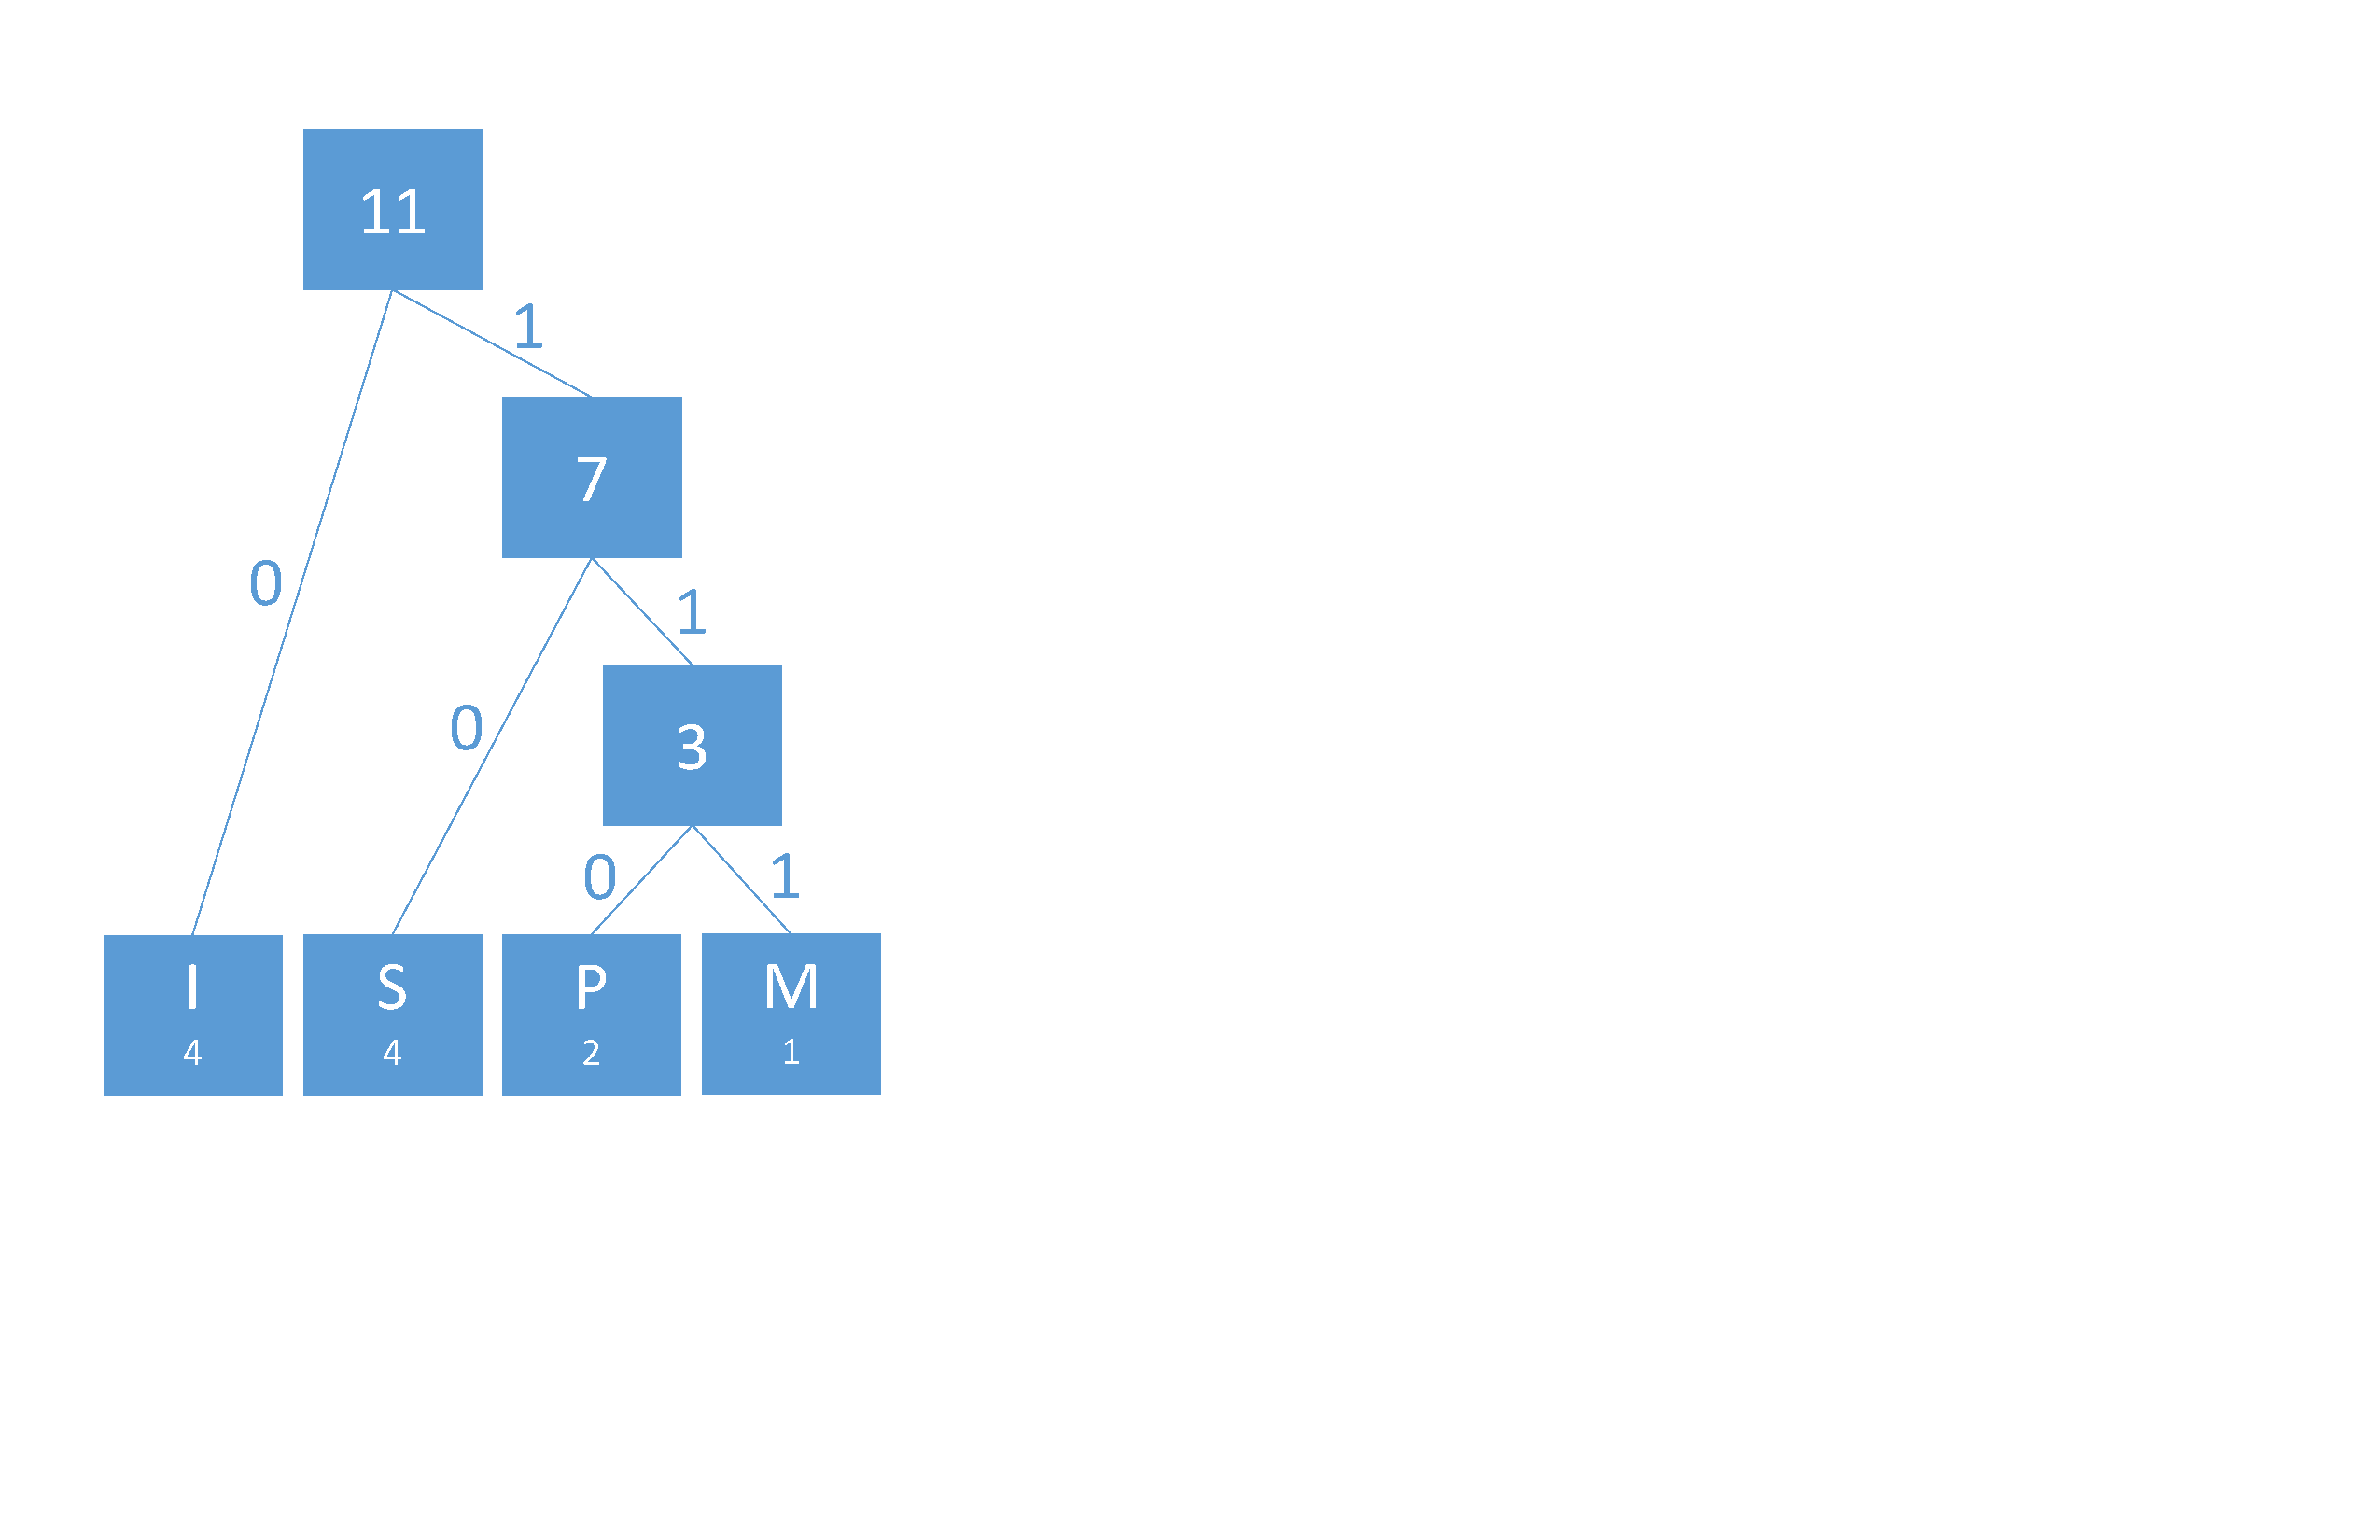
\includegraphics[trim=50 220 770 60, clip, angle=0, width=60mm]{semiHuffman}
\caption{Strom vytvořený při semiadaptivním Huffmanově kódování}
\label{semiHuffmanStrom}
\end{figure}

\begin{table}[!htb]
\centering
\begin{tabular}{|c|c|l|}
\hline
Zdrojový znak & Četnost výskytu & Kódové slovo\\
\hline
I & 4 & 0\\
S & 4 & 10\\
P & 2 & 110\\
M & 1 & 111\\
\hline
\end{tabular}
\caption{Kódová slova semiadaptivního Huffmanova kódu}
\label{semiHuffmanTabulka}
\end{table}

\section{Adaptivní Huffmanovo kódování}
Adaptivní Huffmanovo kódování konstruuje strom při kompresi i dekompresi posloupností stejných kroků, tzv. mirroring. Strom je v každém kroku upraven tak, aby produkoval nejkratší kód pro do té doby zpracovanou část dat. Jak se strom mění, mění se i kódy přiřazené jednotlivým symbolům. Listy stromu obsahují symboly a jejich četnosti výskytu, vnitřní uzly obsahují kumulovanou četnost svých potomků.

Implementovaných verzí existuje několik. Níže je představena verze, kterou navrhl Jeffrey S. Vitter a ve které všechny uzly navíc obsahují pořadové číslo, které je využito při rozhodování při aktualizaci stromu. Také se zde využívají tzv. bloky -- množiny uzlů se stejnou četností. Diagram aktualizace stromu po přečtení jednoho symbolu je možné vidět v příloze \textcolor{red}{odkaz}, způsob kódování, resp. dekódování zprávy na diagramu \textcolor{red}{odkaz}, resp. \textcolor{red}{odkaz}.

Algoritmus začíná pouze s uzlem označeným NYT (not yet transmitted), který symbolizuje všechny znaky, které se zatím ve stromu nevyskytují. Je-li ke zpracování načten symbol, který se ještě ve stromě nevyskytuje, je do výstupu vypsáno kódové slovo uzlu NYT následované nezakódovaným a dohodnutým tvarem zpracovávaného symbolu. Následně se z uzly NYT stane vnitřní uzel a jsou mu přiřazeny dva noví potomci: nový uzel NYT a list reprezentující právě zpracovávaný znak. Poté je strom aktualizován. Je-li ke zpracování načten ve stromě již obsažený symbol, je na výstup vypsáno pouze kódové slovo tohoto symbolu a strom je aktualizován.

Nezakódovaný tvar zpracovávaného symbolu může být například jeho osmibitový ASCII kód. Má-li zdrojová abeceda $\{a_1, a_2, \ldots, a_m\}$ počet znaků roven $m$, pak zvolíme $e,r$ tak, aby splňovala $m= 2^e + r$ a $0 \leq r < 2^e$. Znak $a_k$ poté kódujeme jako $(e+1)$--bitovou reprezentaci čísla $k-1$, je-li $1 \leq k \leq 2r$, jinak je $a_k$ kódován jako $e$--bitová reprezentace čísla $k-r-1$. \cite{dataCompression}, \cite{introductionToDataCompression}

\subsection{Vzorový příklad}
Pokusme se znovu zakódovat slovo MISSISSIPPI, kde budeme uvažovat anglickou abecedu jako zdrojovou. Ta má 26 znaků, tedy $m=26$, $e = 4$ a $r=10$ a znaky číslujeme $a_1 = \mathrm{A}$, $a_2 = \mathrm{B}$ atd.

\subsubsection{Zakódování zprávy a vytvoření stromu}
Začínáme se stromem, který obsahuje pouze kořen NYT. Čteme znak M a na výstup zapíšeme jeho pětibitový nezakódovaný tvar pro $k=13$, tedy \texttt{01100}. Aktualizujeme strom. Čteme znak I, který se ve stromě také nevyskytuje. Na výstup zapíšeme kód uzlu NYT (nyní je to \texttt{0}) a pětibitový nezakódovaný tvar pro $k=9$, tedy \texttt{01000}. Aktualizujeme strom. Dále čteme nový znak S. Na výstup zapíšeme kód uzlu NYT (nyní je to \texttt{00}) a pětibitový nezakódovaný tvar pro $k=19$, tedy \texttt{10010}. Aktualizujeme strom. Dále čteme znak S, který ve stromu již je a tedy vypíšeme pouze jeho kód. Aktualizujeme strom. A tak pokračujeme pro všechny znaky slova.

Výsledný strom je zobrazen na obrázku \ref{adaptivniHuffmanStrom}, celý postup vytvoření stromu pak v příloze \textcolor{red}{odkaz}.

\begin{figure}[!htb]
\centering
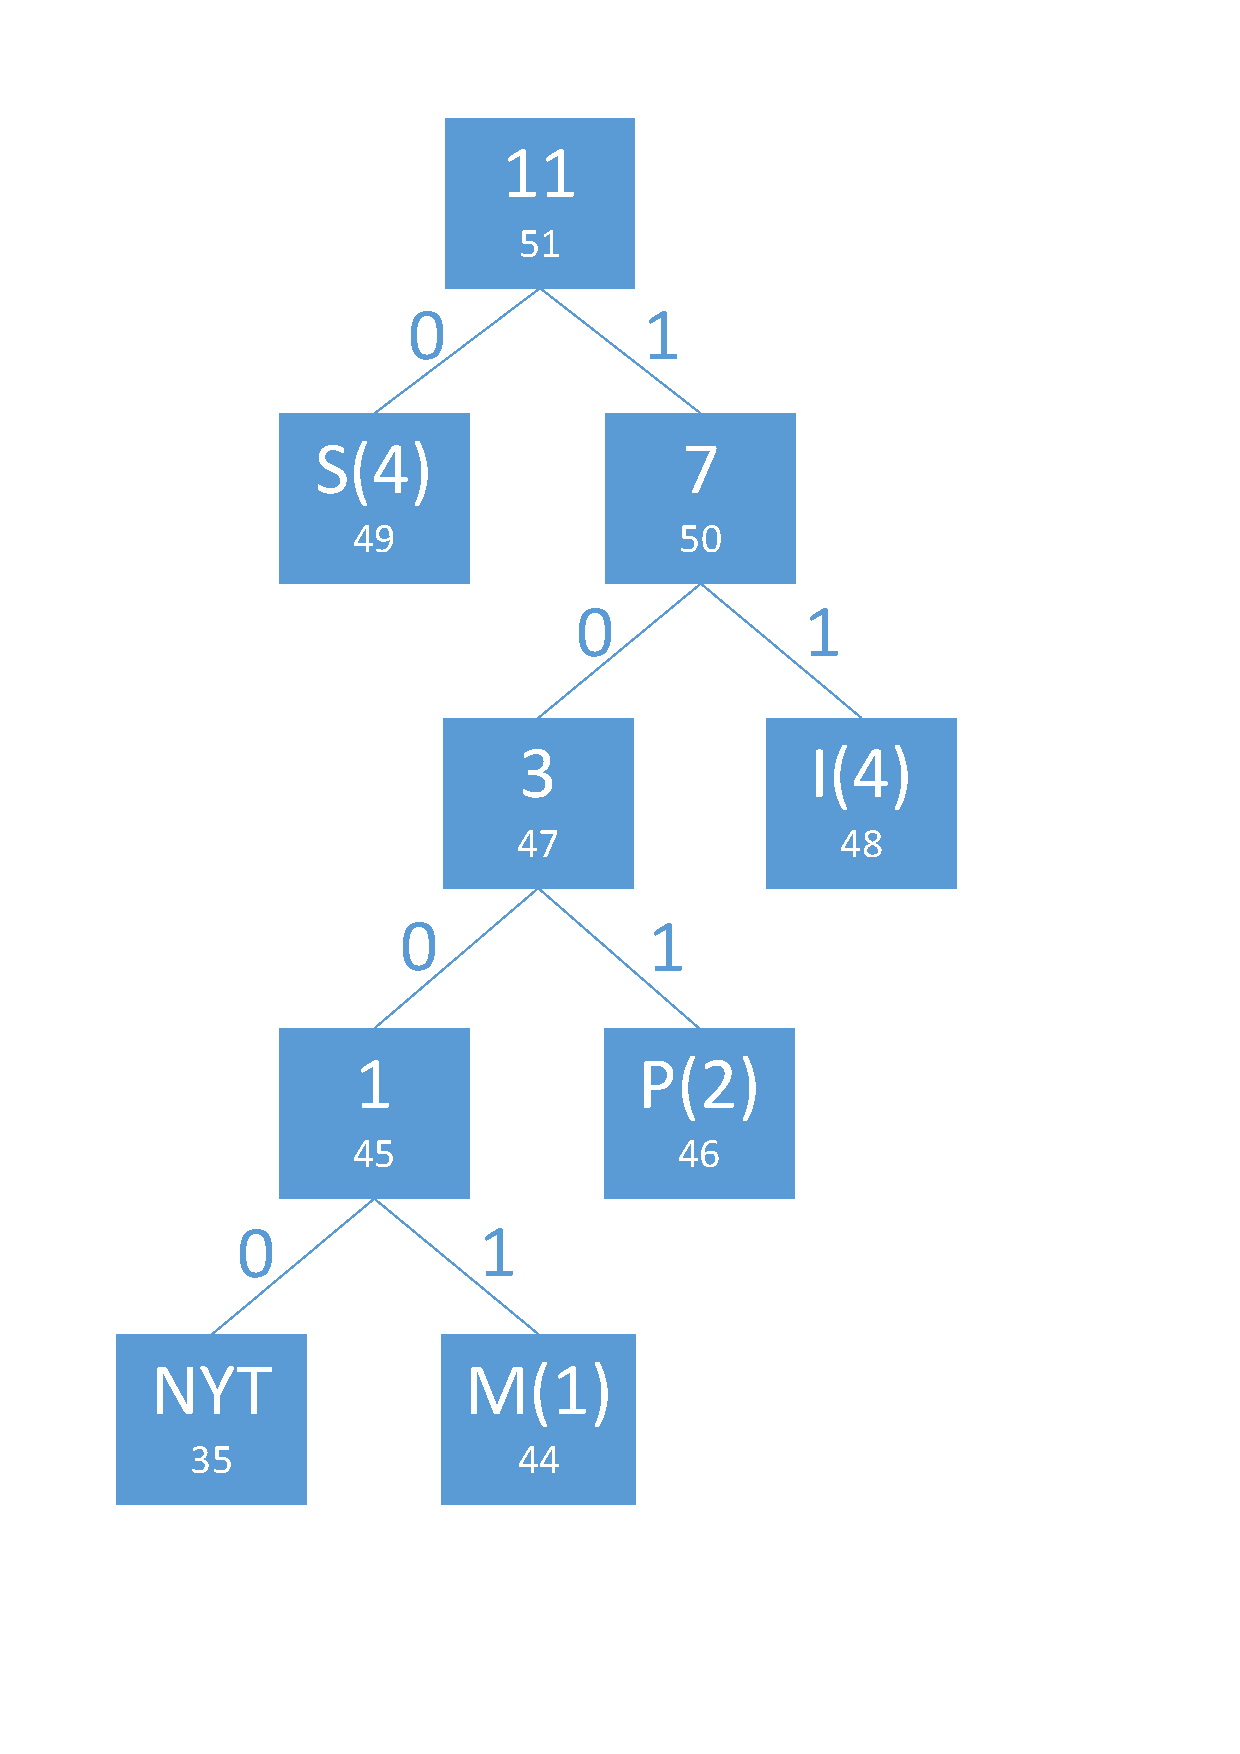
\includegraphics[trim=50 100 130 50, clip, angle=0, width=60mm]{adaptHuffman}
\caption{Strom vytvořený při aptivním Huffmanově kódování}
\label{adaptivniHuffmanStrom}
\end{figure}

\subsubsection{Zakódovaná zpráva}
Výsledná zakódovaná zpráva je tvaru \texttt{01100|0|01000|00|10010|101|11|0|1|01|000|01111|1001|11}, kde jsem pro přehlednost vložil oddělovač \uv{\texttt{|}} oddělující jednotlivé významné bloky.

\subsection{Dekódování zprávy}
Přečteme $e=4$ bitů znaků, jejich hodnota jakožto čtyřbitového čísla je 6, což je menší než $r=10$. Přečteme další znak, hodnota tohoto pětibitového čísla je 12 a tedy jsme přečetli symbol $a_{13} = \mathrm{M}$. Aktualizujeme strom. Následuje 0, která je kódovým slovem pro uzel NYT, po něm vždy následuje nezakódovaný symbol. Obdobně jako pro M přečteme symbol $a_8 = \mathrm{I}$. Aktualizujeme strom. Následuje kódové slovo uzlu NYT a symbol $a_{19} = \mathrm{S}$. Dále čteme kódové slovo uzlu pro symbol S. Takto pokračujeme až do konce zakódované zprávy.

\section{Aritmetické kódování}
  % Popis existujících kompresních algoritmů
\chapter{Přehled existujících implementací kompresních algoritmů pro efektivní uchovávání dat ve formátu XML a JSON}  % Přehled existujících kompresních algoritmů pro efektivní uchovávání dat ve formátech XML a JSON
\chapter{Existující algoritmy pro kompresi XML}
\label{kapitolaXmlAlgoritmy}

Algoritmy anglicky nazývané XML aware s výhodou využívají znalost vnitřní struktury XML formátu. Díky tomu dokáží data předpřipravit tak, aby byla komprese co nejefektivnější. Pro kompresi samotnou jsou používány algoritmy již zmiňované v kapitolách \ref{kapitolaStatistickaKomprese} a \ref{kapitolaSlovnikovaKomprese} a jejich upravené varianty.

XML aware algoritmy můžeme rozdělit dle několika kritérií a to zda podporují dotazování a přístup do komprimovaných dat a nebo zda je nebo není dekompresní algoritmus závislý na přístupu k XML schématu. Z druhé skupiny je častější použití algoritmů, které jsou na schématu nezávislé, protože pro dekompresi není vždy možné přístup ke schématu zaručit.

\section{XMill}
Algoritmus XMill, který nepodporuje dotazování do zkomprimovaných dat, představili pánové Hartmut Liefke a Dan Suciu v roce 2000. Jeho architektura využívá knihovnu kompresních algoritmů zlib, specifické kompresory pro určitý typ dat a navíc podporuje použití kompresorů vytvořených uživatelem pro speciální typy dat. Rozhodnutí, který kompresní algoritmus bude použit, je provedeno na základě znalosti tagů. Architektura algoritmu XMill je postavena na třech základních principech \cite{xmill}:

\begin{description}
\item[Oddělení struktury od dat] Struktura XML složená z tagů a atributů tvoří strom. Data, obsah elementů a hodnoty atributů, jsou reprezentovány jako řetězce. Stromová struktura a data jsou komprimovány odděleně.
\item[Seskupení dat stejného významu] Datové položky stejných elementů jsou seskupeny do jednoho kontejneru a každý kontejner je komprimován odděleně.
\item[Aplikace sémantické komprese] Dle typu dat (text, číslo apod.) je pro kompresi kontejneru použit vhodný kompresní algoritmu, tzv. sémantický kompresor.
\end{description}

\subsection{Popis architektury}
Architektura algoritmu XMill je zobrazena na obrázku \ref{architekturaXMill}. XML dokument je nejprve zpracován pomocí SAX\footnote{Simple API for XML.} parseru, který každý prvek pošle do Path procesoru. Path procesor rozhodne, do kterého existujícího kontejneru prvek vloží, nebo zda nemá vytvořit kontejner nový. Ke každému kontejneru může být uživatelem přiřazen sémantický kompresor a to buď atomický implementovaný v XMill, kombinace atomických pro komplexnější typy a nebo vlastní. Kontejnery jsou plněny až do předem určené velikosti (defaultně je to 8 MB), je-li tato velikost dosažena, je kontejner zkomprimován pomocí gzip\footnote{GNU zip, software pro kompresi dat.}, uložen na disk a komprese dále pokračuje. Díky tomu jsou data rozdělena do vzájemně nezávislých bloků.


\begin{figure}[!htb]
\centering
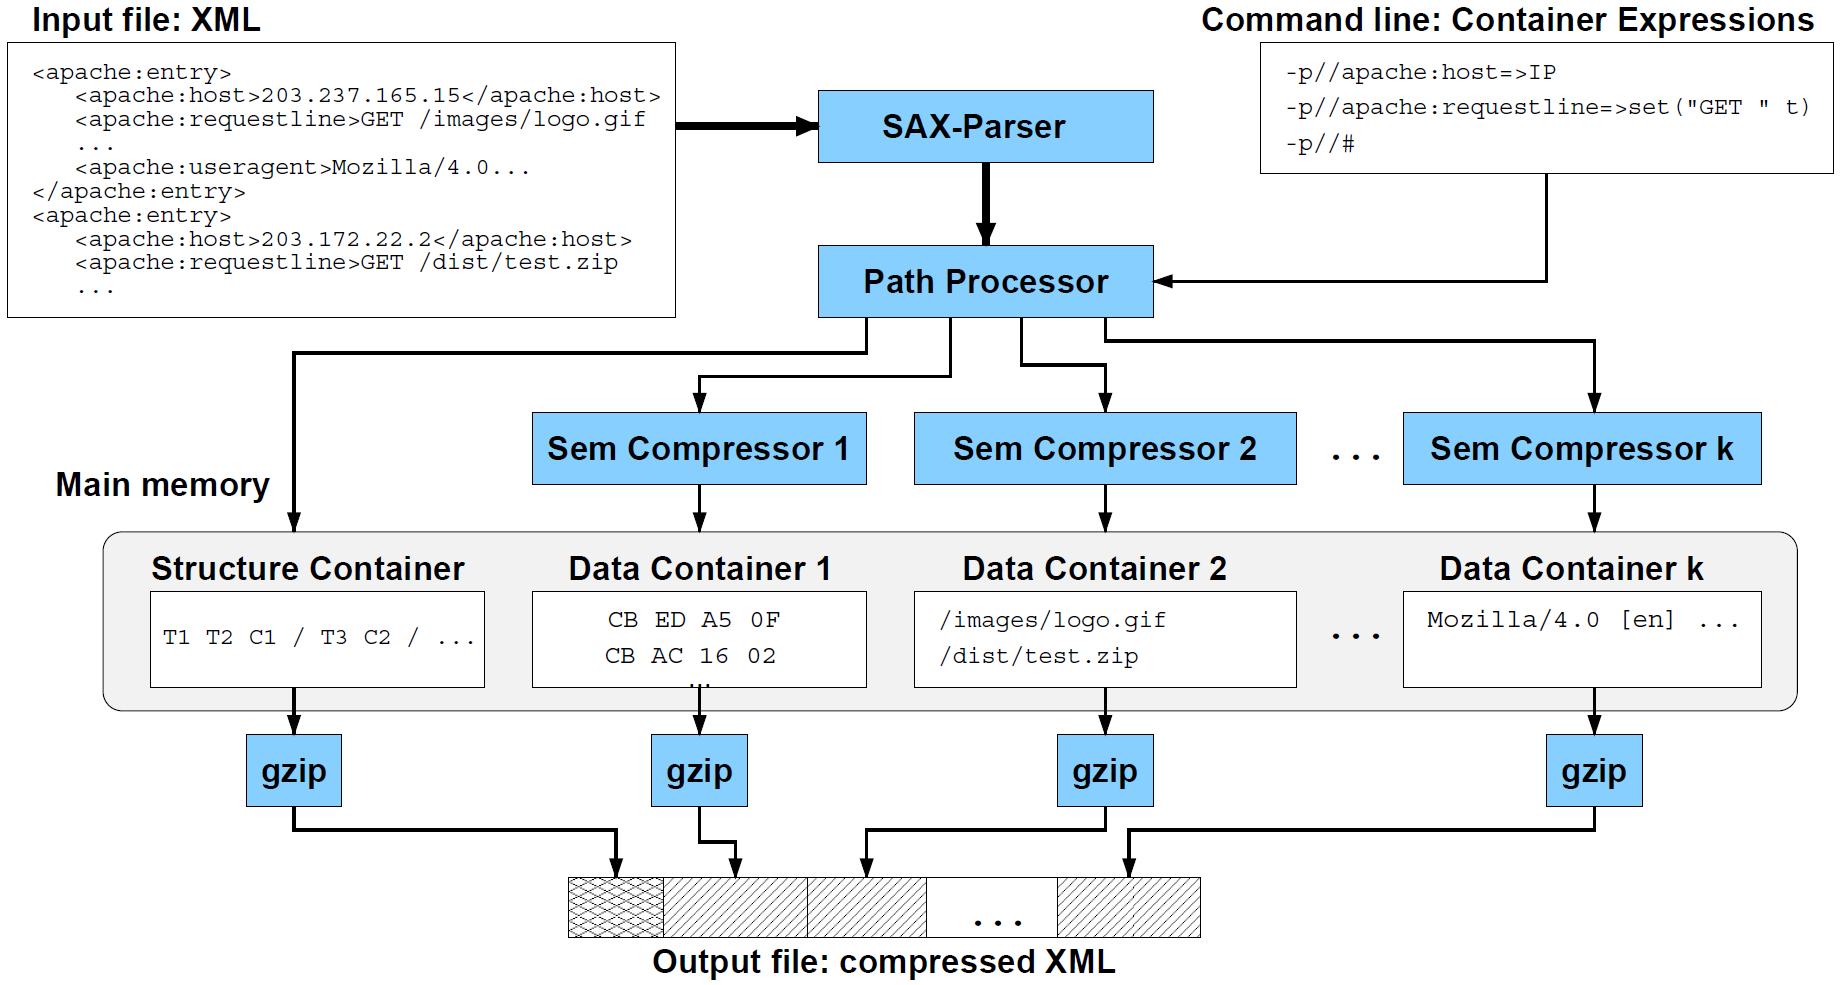
\includegraphics[clip, angle=0, width=150mm]{ArchitekturaXMill}
\caption{Architektura algoritmu XMIll \cite{xmill}}
\label{architekturaXMill}
\end{figure}

\subsection{Oddělení struktury od dat}
\label{xmillOddeleniStruktury}
Struktura XML je složena z tagů a atributů. Počáteční tagy a atributy jsou kódovány slovníkovou metodou a nahrazeny indexem ve slovníku, kladným celým číslem. Ukončující tag je kódován hodnotou 0, při kompresi je díky syntaxi vždy zřejmé, který tak je ukončován. Datové hodnoty jsou nahrazeny záporným indexem kontejneru, do kterého byly přiřazeny.\cite{xmill}

Pro příklad zpracujeme následující informace o článku:

\begin{verbatim}
<article mdate="2011-01-11" key="journals/acta/GoodmanS83">
  <author>
    <name>Nathan Goodman</name>
    <title>Mr.</title>
  </author>
  <title>NP-complete Problems Simplified on Tree Schemas.</title>
</article>
\end{verbatim}

Tagy zde jsou \texttt{article}, \texttt{author} a \texttt{title} a atributy \texttt{mdate} a \texttt{key}. Po zpracování dostaneme výstup \texttt{1 2 -3 3 -4 0 4 5 -5 0 6 -6 0 0 7 -7 0 0}. Lze si povšimnout, že indexování kontejnerů začíná až číslem 3, to proto, že index 0 je rezervován pro kontejner struktury, 1 pro kontejner bílých znaků (umožňuje zachování formátovacích mezer) a 2 pro kontejner obsahující procesní instrukce, DTD a jiné.

\subsection{Seskupení dat stejného významu}
Mapování mezi daty a kontejnery provádí Path procesor na základě cesty k datům (path) a na uživatelem definovaném regulárním výrazu container expression. Základní myšlenkou je hodnotám pro každý tag nebo atribut přiřadit vlastní kontejner. Cesta k datům v příkladě z předchozí části \ref{xmillOddeleniStruktury} vypadá například \texttt{/article/@key} pro atribut a \texttt{/article/author/name} pro tag. Pomocí container expression je možné nastavit pravidla, kdy budou například hodnoty různých tagů ukládány do stejného kontejneru.\cite{xmill}

\subsection{Sémantická komprese}
Jak již bylo zmíněno v úvodu popisu tohoto algoritmu, jsou podporovány 3 druhy sémantických kompresorů: atomické, kombinované a definované uživatelem. Atomických kompresorů je 8, například textový kompresor \texttt{t}, který řetězec pouze zkopíruje na výstup (ten bude později zkomprimován pomocí gzip), nebo kompresor \texttt{u}, který komprimuje kladná celá čísla.

Kombinovaný kompresor je vhodný pro hodnoty, ve kterých lze nalézt nějaký vzor nebo strukturu. Jako příklad lze uvést sekvenční kompresor pro kompresi IP adresy \texttt{seq(u8 "." u8 "." u8 "." u8)}, což znamená sekvenci čtyř kladných celých čísel menších než 256 oddělených tečkou.

Vlastní kompresory lze s výhodou použít na data, která mají strukturu složitou nebo velmi těžce vyjádřitelnou pomocí kombinovaných kompresorů. Autoři jako příklad takových dat uvádějí DNA sekvence. Aby bylo možné data komprimovaná za pomocí vlastní kompresorů zpětně rekonstruovat, musí mít dekompresní algoritmus samozřejmě také přístup k použitému vlastnímu kompresoru.\cite{xmill}  % Vlastní implementace vybraných kompresních algoritmů
\chapter{Existující algoritmy pro kompresi JSON}
%nalezení a odstranění redundance
%zanedbání formátovacích mezer a tabulátorů
%json po kompresi je zase validní json!



\label{kapitolaSpecifickeAlgoritmy}

JSON byl navržen jako odlehčená varianta způsobu formátování dat proti XML, čímž byla odstraněna i redundance při použití počátečního a ukončovacího tagu. Po seznámení s jeho definicí a syntaxí je zřejmé, že zde již nezbývá moc prostoru k dalšímu odlehčení. Podíváme-li se ale na data zapsaná v tomto formátu, která mohou obsahovat například výstup SQL příkazu SELECT nad databází (viz \textcolor{red}{odkaz na testovací soubor na přiloženém CD}), můžeme vidět, že se zde některé prvky přeci jen opakují. Jsou to klíče, včetně uvozovek, v jednotlivých objektech, které stačí zapsat pouze jednou. Tohoto poznatku využívají i dva vybrané algoritmy JSONH a CJSON. Rád bych čtenáře upozornil, že algoritmů pro kompresi JSON neexistuje mnoho, resp. jsou si velice podobné myšlenkou, provedením i názvy.

S daty v tomto formátu nepracujeme jako s obyčejným textem, ale převedeme je na kolekci instancí tříd, které reprezentují. V rychlosti tohoto zpracování vyniká především JavaScript. 

\section{JSONH}
Tento algoritmus dovoluje komprimovat pouze homogenní kolekce dat, v terminologii JSON jde o pole objektů, které mají stejný počet klíčů se stejnými názvy. Homogenitu dat musí zaručit uživatel, algoritmus samotný toto nikterak neošetřuje. Autoři projektu JSONH, kde je algoritmus implementován, na serveru github.com uvádějí, že data mohou být v některých případech zmenšena až na 30 \%.

\subsection{Vzorová data}
Mějme homogenní kolekci zaměstnanců firmy, ve které máme uložené databázové id, příjmení a pozici, na které zaměstnanec pracuje. Tato kolekce může vypadat následujícím způsobem.

\texttt{[\\
\hspace*{5mm}\{ \textquotedblright id\textquotedblright : 1, \textquotedblright name\textquotedblright : \textquotedblright Sánchez\textquotedblright, \textquotedblright position\textquotedblright : \textquotedblright Manager\textquotedblright\ \},\\
\hspace*{5mm}\{ \textquotedblright id\textquotedblright : 2, \textquotedblright name\textquotedblright : \textquotedblright Duffy\textquotedblright, \textquotedblright position\textquotedblright : \textquotedblright Programmer\textquotedblright\ \},\\
\hspace*{5mm}\{ \textquotedblright id\textquotedblright : 3, \textquotedblright name\textquotedblright : \textquotedblright Tamburello\textquotedblright, \textquotedblright position\textquotedblright : \textquotedblright Worker\textquotedblright\ \}\\
]}

\subsection{Postup komprese}
\begin{enumerate}
\item Textová data jsou převedena na pole objektů.
\item \label{jsonhItem0} Z prvního objektu v poli jsou určeny klíče a jejich počet.
\item \label{jsonhItem1} Ze všech objektů v poli jsou postupně vyzvednuty hodnoty pro příslušné klíče, přičemž je zachováno pořadí klíčů, jak jsme jej získali v kroku \ref{jsonhItem0}.
\item Je vytvořeno pole, které obsahuje prvky: počet klíčů, seznam klíčů a hodnoty vyzvednuté v kroku \ref{jsonhItem1}.
\item Vytvořené pole serializujeme jako JSON do řetězce nebo souboru.
\end{enumerate}

\subsection{Data po kompresi}
\texttt{[ 3, \textquotedblright id\textquotedblright, \textquotedblright name\textquotedblright, \textquotedblright position\textquotedblright, 1, \textquotedblright Sánchez\textquotedblright, \textquotedblright Manager\textquotedblright, 2, \textquotedblright Duffy\textquotedblright,\\
\hspace*{5mm}\textquotedblright Programmer\textquotedblright, 3, \textquotedblright Tamburello\textquotedblright, \textquotedblright Worker\textquotedblright\ ]}

\subsection{Postup rekonstrukce dat}
\begin{enumerate}
\item Textová data jsou převedena na pole hodnot.
\item Z prvního prvku v poli určíme počet klíčů, označíme $n$.
\item Z 2. až $(n+1)$--ního prvku určíme klíče.
\item Z následujících prvků (po $n+1$) rekonstruujeme původní objekty až do konce pole a ukládáme je do pole nového.
\item Nové pole serializujeme jako JSON do řetězce nebo souboru.
\end{enumerate}

\section{CJSON}
Proti JSONH dokáže algoritmus CJSON komprimovat i nehomogenní data. K tomu, aby bylo při kompresi dosaženo významné úspory, je nutná určitá struktura dat. Tu bych přirovnal k dědičnosti, jak ji známe z principů objektově orientovaného programování. To znamená, že data lze popsat pomocí tříd, které sdílejí některé členy. Účinnost komprese závisí na poměru počtu tříd a množství dat k nim příslušných. Platí, že čím menší počet tříd a větší množství příslušných dat, tím větší je kompresní účinnost. Za ideál lze potom považovat homogenní data, tedy případ kdy stačí k popisu pouze jedna třída, ke které přísluší všechna data.

Algoritmus v průběhu komprese vytváří postupně strom šablon, který je na závěr vložen do výstupu ve formě jednotlivých šablon, která využívá již zmiňované dědičnosti. Konstrukce stromu je zobrazena na obrázku \ref{cjsonKonstrukceStromu}. \textcolor{red}{Doplnit očíslování v obrázku a popis vytváření stromu.}

\begin{figure}[!htb]
\centering
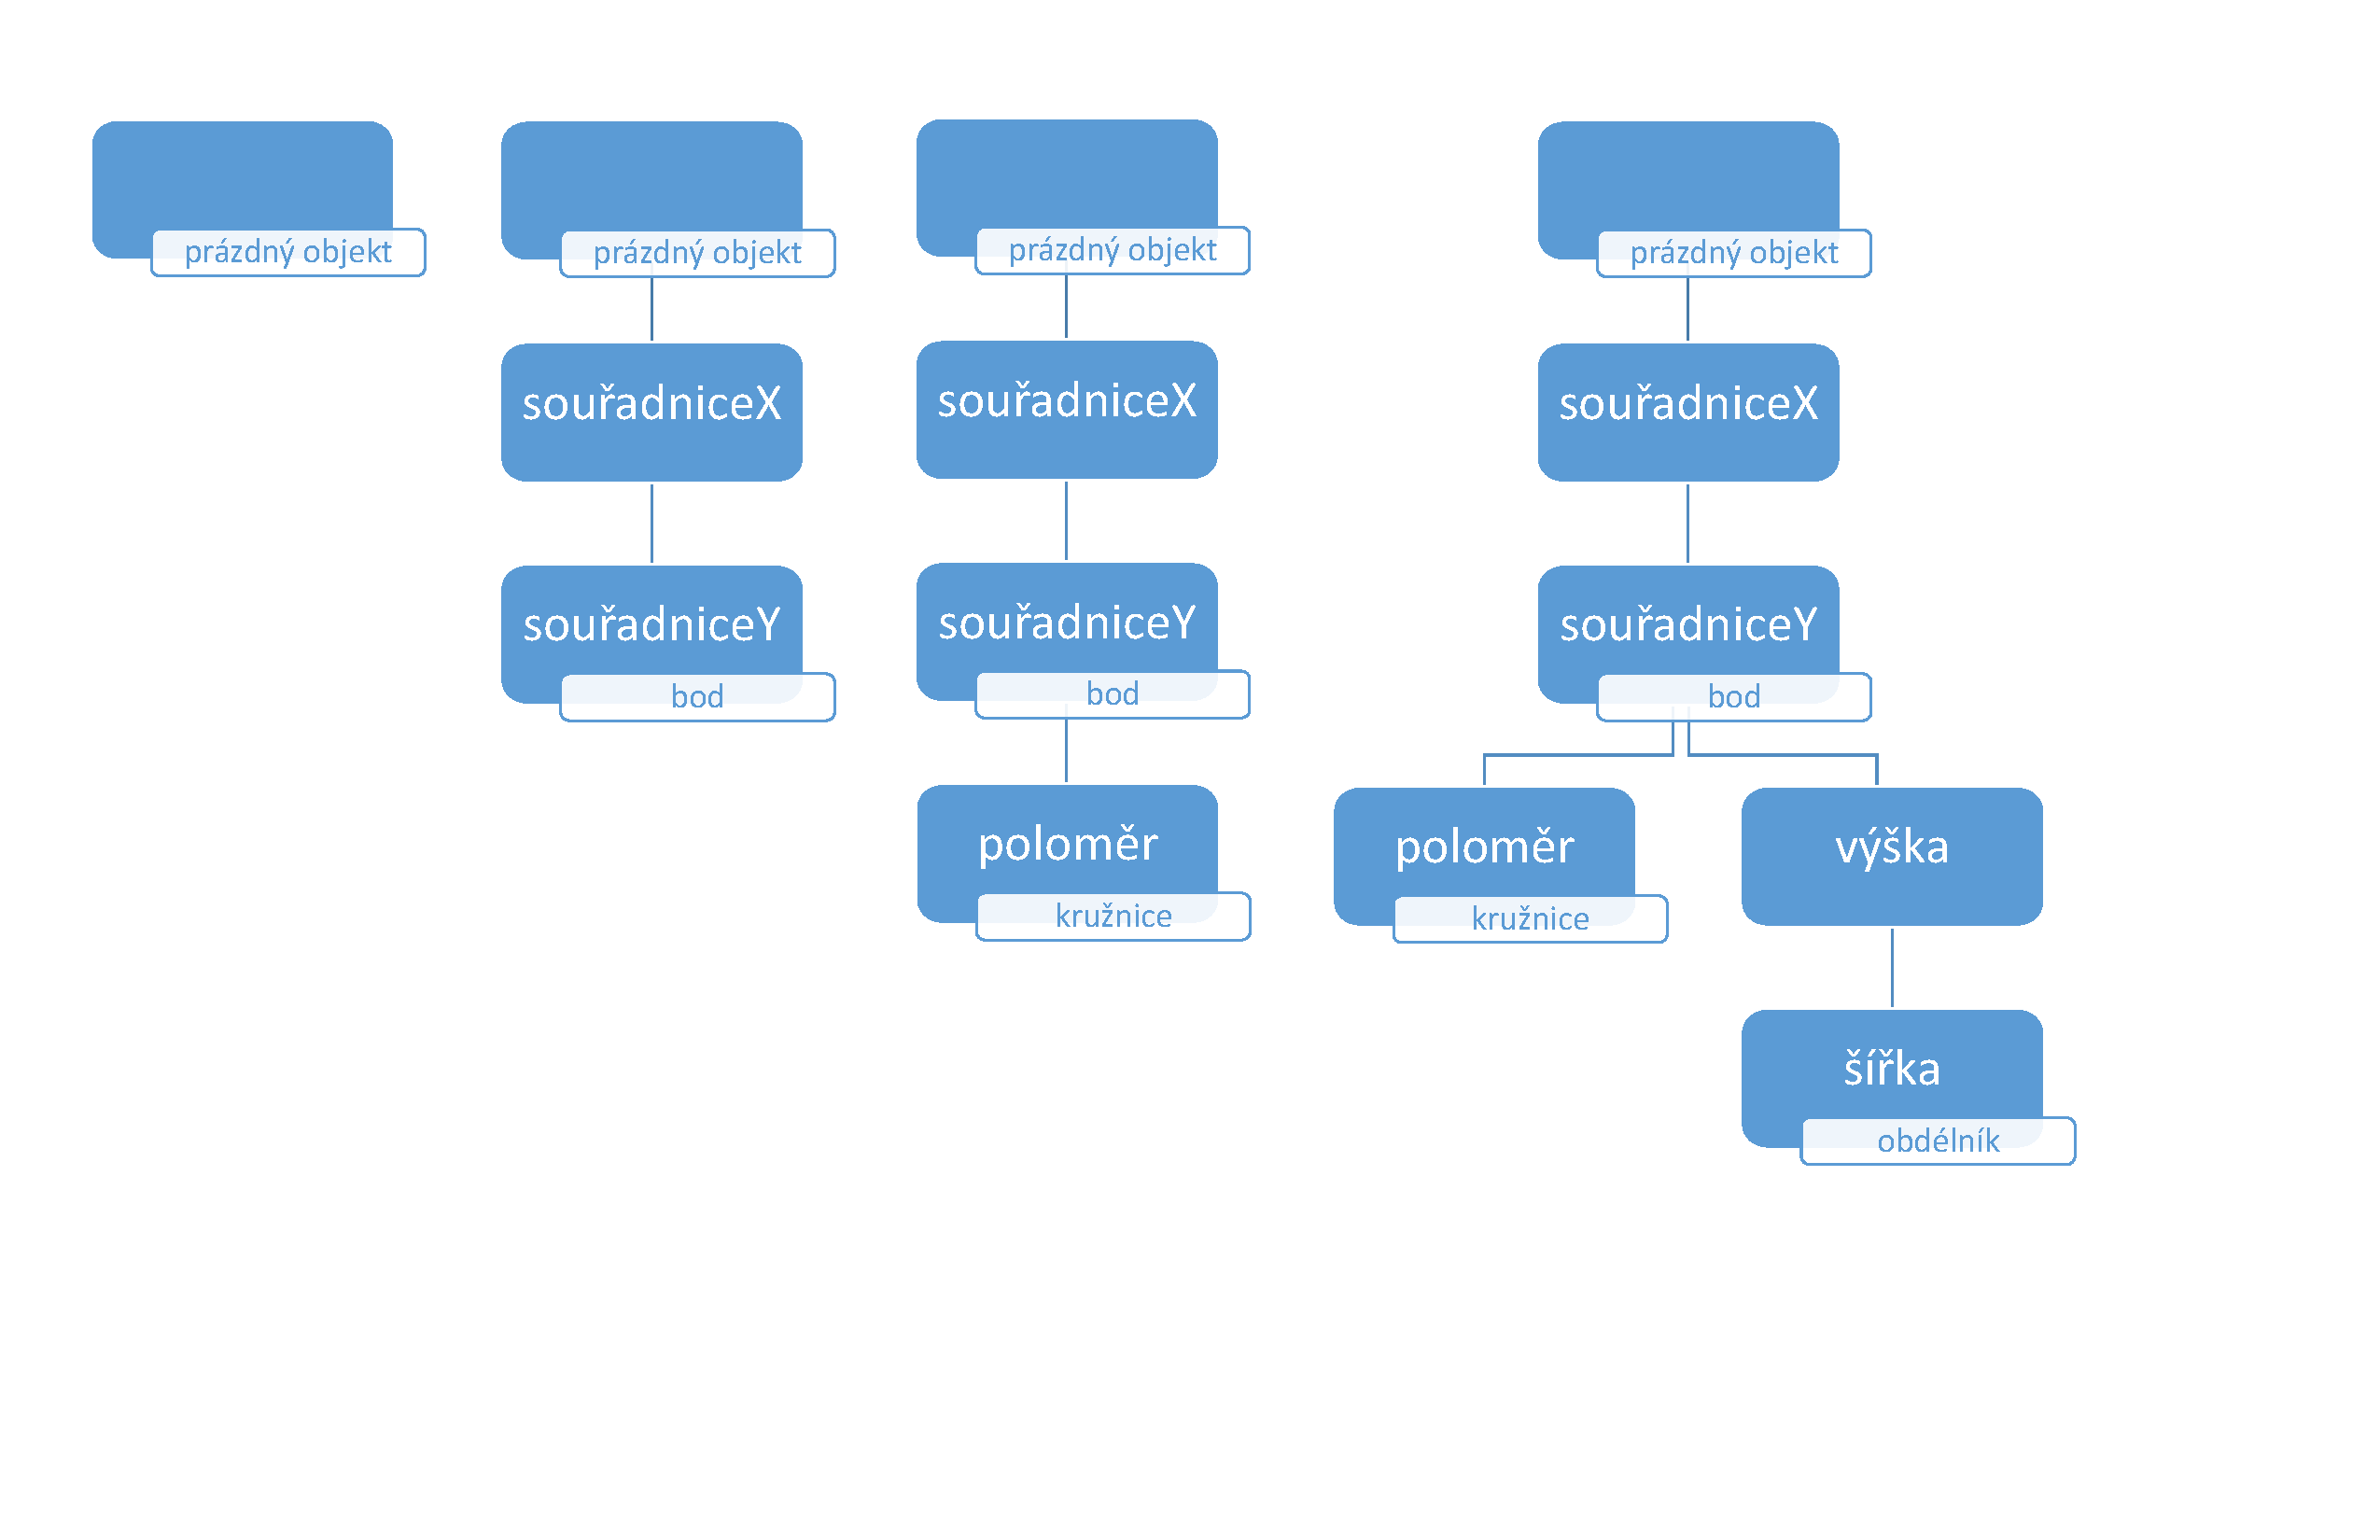
\includegraphics[trim=30 180 150 50, clip, angle=0, width=150mm]{cjsonStrom}
\caption{Postup vytvoření stromu šablon}
\label{cjsonKonstrukceStromu}
\end{figure}

\subsection{Vzorová data}
\textcolor{red}{Vytvořit data, popsat, upravit obrázek konstrukce stromu!!!}

Mějme homogenní kolekci zaměstnanců firmy, ve které máme uložené databázové id, příjmení a pozici, na které zaměstnanec pracuje. Tato kolekce může vypadat následujícím způsobem.

\texttt{[\\
\hspace*{5mm}\{ \textquotedblright id\textquotedblright : 1, \textquotedblright name\textquotedblright : \textquotedblright Sánchez\textquotedblright, \textquotedblright position\textquotedblright : \textquotedblright Manager\textquotedblright\ \},\\
\hspace*{5mm}\{ \textquotedblright id\textquotedblright : 2, \textquotedblright name\textquotedblright : \textquotedblright Duffy\textquotedblright, \textquotedblright position\textquotedblright : \textquotedblright Programmer\textquotedblright\ \},\\
\hspace*{5mm}\{ \textquotedblright id\textquotedblright : 3, \textquotedblright name\textquotedblright : \textquotedblright Tamburello\textquotedblright, \textquotedblright position\textquotedblright : \textquotedblright Worker\textquotedblright\ \}\\
]}

\subsection{Postup komprese}
\begin{enumerate}
\item Textová data jsou převedena na pole objektů.
\item Ze všech objektů v poli jsou postupně vyzvednuty hodnoty a uloženy do nového pole objektů. Tyto objekty obsahují pouze pole příslušných hodnot. Zároveň je konstruován strom šablon.
\item Ze stromu šablon je vytvořeno pole šablon. Šablona je pole obsahující identifikátor šablony, ze které dědí, a klíče. Identifikátor 0 je rezervován pro šablonu odpovídající prázdnému objektu.
\item Objekty s hodnotami jsou doplněny o identifikátor odpovídající šablony.
\item \label{cjsonItem0}Ze vzniklých polí vytvoříme objekt obsahující identifikátor kompresního algoritmu (klíč \texttt{"f"}), pole šablon (klíč \texttt{"t"}) a pole hodnot (klíč \texttt{"v"}) (viz \ref{cjsonPoKompresi}).
\item Objekt vzniklý v bodu \ref{cjsonItem0} serializujeme jako JSON do řetězce nebo souboru.
\end{enumerate}

\subsection{Data po kompresi}
\label{cjsonPoKompresi}
\texttt{\{\hspace*{3mm}"f" : "cjson",\\
\hspace*{5mm}"t" : [ [ 0, "x", "y" ], [ 1, "width", "height" ] ],\\
\hspace*{5mm}"v" : [ \{ "" : [ 1, 100, 100 ] \}, \{ "" : [ 2, 100, 100, 200, 150 ] \} ] \}}

\subsection{Postup rekonstrukce dat}
\begin{enumerate}
\item Textová data jsou převedena na pole hodnot.
\item Vytvoříme pole, do kterého postupně vkládáme objekty vzniklé z prvků pole hodnot a příslušných šablon.
\item Tuto kolekci serializujeme jako JSON do řetězce nebo souboru.
\end{enumerate}  % Porovnání účinnosti komprese dat ve formátech XML a JSON


\chapter*{Závěr} \addcontentsline{toc}{chapter}{Závěr}   % SEM NESAHEJTE!
%V závěru práce byste měli svou práci zhodnotit jako autor. Závěr by tedy měl obsahovat:
%\begin{itemize}
%\item shrnutí výsledků, ke kterým autor dospěl,
%\item přínos autora práce k řešené problematice (co je v práci původní),
%\item zhodnocení využitelnosti dosažených výsledků,
%\item možné pokračování práce (resp. další náměty pro řešení v uvedení oblasti) -- nemusí být řešena Vaší osobou.
%\end{itemize}

%Závěr se většinou vejde na 1 stránku (max. 3 stránky).

Tato závěrečná diplomová práce se věnuje kompresi dat a to hlavně kompresi s využitím znalosti struktury dat. Porovnávány jsou vzájemně datové formáty XML a JSON s cílem určit, který z nich je vhodnější ke kompresi a tím úspornější při archivaci či přenosu dat.

XML je redundantní textový formát, který byl navržen tak, aby byl snadno čitelný pro člověka. Této redundance lze při kompresi XML souboru využít. Formát JSON vznikl jako úsporná alternativa právě ke XML s myšlenkou odstranění redundance dané definicí syntaxe XML. Oba formáty se dnes velice často využívají v prostředí internetu pro práci s daty a proto je vhodné vědět, jaké úspory může jejich komprese přinést.

Praktická část práce je složena ze dvou úkolů. V prvním byla implementována kompresní knihovna, která obsahuje tři algoritmy. Algoritmy Huffmanovo kódování a LZ77 byly zvoleny zejména z toho důvodu, že je úspěšně kombinují algoritmy LZMA2 a gzip, který navíc ke kompresi souborů XML využívá algoritmus XMill. Velmi důležitou součástí implementace kompresního algoritmu je správa paměti, kterou se mi v práci nepodařilo úplně vyřešit.

Dalším praktickým úkolem bylo porovnat účinky komprese dat zapsaných ve formátech XML a JSON pomocí různých kompresních technik. Zvolené algoritmy LZMA2, BZip2, PPMd, gzip, XMILL, JSONH a CJSON byly použity ke komprimaci pěti souborů obsahujících XML a JSON. Tyto soubory byly voleny tak, aby nebyly navzájem podobné velikostí a strukturou dat. Naměřené výsledky jsou v~podobě grafů a tabulky popsány v~kapitole \ref{kapitolaPorovnaniUcinnosti}. Z naměřených dat vyplývá, že moderní kompresní metody, jako jsou LZMA2 a~PPMd, dokáží komprimovat XML i JSON se srovnatelnou nebo dokonce vyšší účinností než algoritmy specializované. Algoritmy JSONH a CJSON dosáhly nejhorších výsledků pro úplně všechny testovací soubory, což je ale dáno naprosto rozdílným způsobem komprimace.

Mezi soubory XML a JSON obsahující stejná data je možné pozorovat významný rozdíl ve velikosti ve prospěch formátu JSON. Toto ale neplatí pro soubory po komprimaci, kdy je rozdíl ve velikosti podstatně menší. Pokud uživatel nevyžaduje možnost práce s~komprimovanými daty, lze doporučit použití klasických běžně dostupných kompresních algoritmů. Na základě výše zmíněných poznatků považuji formát JSON za vhodnější ke kompresi a~práci s daty.  % Závěr, je vkládán z jiného souboru

%  Seznam použitých zdrojů  %%%%%%%%%%%%%%%%%%%%%%
\newpage  % SEM NESAHEJTE!
\renewcommand{\bibname}{Seznam použitých zdrojů} % SEM NESAHEJTE!
\addcontentsline{toc}{chapter}{Seznam použitých zdrojů} % SEM NESAHEJTE!

% !!! Literatura se řadí abecedně.
% !!! Literatura se má seřadit abecedně.
\begin{thebibliography}{99}
\bibitem{json} Standard ECMA-404. {\em The JSON Data Interchange Format.} Geneva: Ecma International, 2013, [online], [cit. 28. října 2014]. Dostupné na: {\tt <http://www.ecma-international.org/publications/files/ECMA-ST/ECMA-404.pdf>}.
\bibitem{idc} The Digital Universe of Opportunities: Rich Data and the Increasing Value of the Internet of Things. INTERNATIONAL DATA CORPORATION. {\em EMC} [online]. 2014 [cit. 2015-02-25]. Dostupné z: {\tt <http://www.emc.com/leadership/digital-universe/2014iview/executive-summary.htm>}.
\bibitem{w3cxml} W3C. {\em Extensible Markup Language (XML) 1.0 (Fifth Edition).} 26. listopadu 2008, [online], [cit. 26. listopadu 2014]. Dostupné na: {\tt <http://www.w3.org/TR/2008/REC-xml-20081126/>}.
\end{thebibliography}
  % text, který je vkládán z jináho souboru, MَŮŽETE ZMĚNIT NÁZEV souboru nebo smazat tento řádek a seznam literatury napsat přímo sem

\newpage % SEM NESAHEJTE!
%  PŘÍLOHY PRÁCE %%%%%%%%%%%%%%%%%%%%%%
\appendix  % přílohy budou opravdu "Přílohy"  :-)     SEM NESAHEJTE!
\addcontentsline{toc}{chapter}{Přílohy} % přidat položku do obsahu      SEM NESAHEJTE!

\part*{Přílohy}  % SEM NESAHEJTE!
\renewcommand{\appendixname}{Příloha} % aby se přílohy nejmenovaly "Dodatek"  SEM NESAHEJTE!

% zde VYMAŽTE NÁZVY vkládaných souborů NEBO sem můžetete rovnou napsat text příloh (a smažte dva následující řádky)

\chapter{Příklady}
\label{prilohaa}

\section{Porovnání XML a JSON}
\label{prilohaPorovnaniXmlJson}
\begin{minipage}{0.5\textwidth}
{\Large XML}\\\\
\texttt{\small
<widget>\\
\hspace*{2mm}<debug>on</debug>\\
\hspace*{2mm}<window\\
\hspace*{4mm}title="Sample Widget\textquotedblright>
\hspace*{4mm}<name>main\_window</name>\\
\hspace*{4mm}<width>500</width>\\
\hspace*{4mm}<height>500</height>\\
\hspace*{2mm}</window>\\
\hspace*{2mm}<image\\
\hspace*{4mm}src="Images/Sun.png"\\
\hspace*{4mm}name="sun1\textquotedblright>\\
\hspace*{4mm}<hOffset>250</hOffset>\\
\hspace*{4mm}<vOffset>250</vOffset>\\
\hspace*{4mm}<alignment>center</alignment>\\
\hspace*{2mm}</image>\\
\hspace*{2mm}<text\\
\hspace*{4mm}data="Click Here"\\
\hspace*{4mm}size="36"\\
\hspace*{4mm}style="bold\textquotedblright>\\
\hspace*{4mm}<name>text1</name>\\
\hspace*{4mm}<hOffset>250</hOffset>\\
\hspace*{4mm}<vOffset>100</vOffset>\\
\hspace*{4mm}<alignment>center</alignment>\\
\hspace*{4mm}<onMouseUp>sun1.opacity =\\
\hspace*{6mm}(sun1.opacity / 100) * 90;\\
\hspace*{4mm}</onMouseUp>\\
\hspace*{2mm}</text>\\
</widget>}
\end{minipage}
\begin{minipage}{0.5\textwidth}
{\Large JSON}\\\\
\texttt{\small
\{ "widget": \{\\
\hspace*{6mm}"debug": "on",\\
\hspace*{6mm}"window": \{\\
\hspace*{8mm}"title": "Sample Widget",\\
\hspace*{8mm}"name": "main\_window",\\
\hspace*{8mm}"width": 500,\\
\hspace*{8mm}"height": 500\\
\hspace*{6mm}\},\\
\hspace*{6mm}"image": \{\\ 
\hspace*{8mm}"src": "Images/Sun.png",\\
\hspace*{8mm}"name": "sun1",\\
\hspace*{8mm}"hOffset": 250,\\
\hspace*{8mm}"vOffset": 250,\\
\hspace*{8mm}"alignment": "center"\\
\hspace*{6mm}\},\\
\hspace*{6mm}"text": \{\\
\hspace*{8mm}"data": "Click Here",\\
\hspace*{8mm}"size": 36,\\
\hspace*{8mm}"style": "bold",\\
\hspace*{8mm}"name": "text1",\\
\hspace*{8mm}"hOffset": 250,\\
\hspace*{8mm}"vOffset": 100,\\
\hspace*{8mm}"alignment": "center",\\
\hspace*{8mm}"onMouseUp": "sun1.opacity =\\
\hspace*{10mm}(sun1.opacity / 100) * 90;"\\\\
\hspace*{6mm}\}\\
\}\}
}
\end{minipage} % příloha 1: vložená z externího souboru
%\chapter{Obsah CD}
\label{prilohab}

Adresáře na CD a jejich obsah:

\begin{description}
\item [Prace] – obsahuje textovou a obrazovou část bakalářské práce včetně všech příloh ve formátu PDF.
\item [Projekt] – obsahuje zdrojové kódy knihovny vytvořené ve vývojovém prostředí MS Visual Studio 2013 a použité externí knihovny.
\item [Knihovna] - obsahuje vytvořenou DLL knihovnu.
\end{description} % příloha 2: vložená z externího souboru

\end{document} % SEM NESAHEJTE!